% ****** Start of file apssamp.tex ******
%
%   This file is part of the APS files in the REVTeX 4.1 distribution.
%   Version 4.1r of REVTeX, August 2010
%
%   Copyright (c) 2009, 2010 The American Physical Society.
%
%   See the REVTeX 4 README file for restrictions and more information.
%
% TeX'ing this file requires that you have AMS-LaTeX 2.0 installed
% as well as the rest of the prerequisites for REVTeX 4.1
%
% See the REVTeX 4 README file
% It also requires running BibTeX. The commands are as follows:
%
%  1)  latex apssamp.tex
%  2)  bibtex apssamp
%  3)  latex apssamp.tex
%  4)  latex apssamp.tex
%
\documentclass[%
%%%%%ok reprint,
%superscriptaddress,
%groupedaddress,
%unsortedaddress,
%runinaddress,
%frontmatterverbose, 
preprint,
%showpacs,preprintnumbers,
nofootinbib,
%nobibnotes,
%bibnotes,
 amsmath,amssymb,
 aps,
%pra,
%prb,
%rmp,
%prstab,
%prstper,
floatfix,
]{revtex4-1}

\usepackage{graphicx}% Include figure files
\usepackage{setspace}
\usepackage{dcolumn}% Align table columns on decimal point
\usepackage{bm}% bold math
%\usepackage[caption=false]{subfig}% bold math
\usepackage{subcaption}% bold math
%\usepackage{hyperref}% add hypertext capabilities
%\usepackage[mathlines]{lineno}% Enable numbering of text and display math
%\linenumbers\relax % Commence numbering lines

%\usepackage[showframe,%Uncomment any one of the following lines to test 
%%scale=0.7, marginratio={1:1, 2:3}, ignoreall,% default settings
%%text={7in,10in},centering,
%%margin=1.5in,
%%total={6.5in,8.75in}, top=1.2in, left=0.9in, includefoot,
%%height=10in,a5paper,hmargin={3cm,0.8in},
%]{geometry}

\begin{document}

\preprint{draft}

\title{ 
Transition Radiation Detector for the GlueX experiment
}% Force line breaks with \\
%\thanks{Thanks to everybody who contributed to this work}%
\author{Alexander Austregesilo}
\author{Eugene Chudakov}
\author{Sergey Furletov}
\author{Lubomir Pentchev}
\affiliation{Thomas Jefferson National Accelerator Facility, Newport News, Virginia 23606, USA}
\author{Sean Dobbs}
\affiliation{Florida State University, Tallahassee, Florida 32306, USA}
%
%\author{Ann Author}
% \altaffiliation[Also at ]{Physics Department, XYZ University.}%Lines break automatically or can be forced with \\
%\author{Second Author}%
% \email{Second.Author@institution.edu}
%\affiliation{%
% Authors' institution and/or address\\
% This line break forced with \textbackslash\textbackslash
%}%

%\collaboration{GlueX Collaboration}%\noaffiliation


\date{\today}% It is always \today, today,
             %  but any date may be explicitly specified

\begin{abstract}
We propose to build a Transition Radiation Detector (TRD) 
with Gaseous Electron Multiplier (GEM) amplification, referred as GEM-TRD,
to improve the electron-pion separation in the GlueX experiment.
It will allow to study precisely reactions with 
electron-positron pairs in the final states; such reactions like
$J/\psi $ photoproduction near threshold have significant impact
in many fields of the particle physics.
The document discusses the motivation for such an upgrade 
and the physics goals, together with  the
technical description of the proposed detector and the electronics. 
Requirements for the GEM-TRD gas system are specified. 
Finally, estimates of the costs and the proposed time line are presented.
\end{abstract}

%\pacs{Valid PACS appear here}% PACS, the Physics and Astronomy
%                             % Classification Scheme.
%%\keywords{Suggested keywords}%Use showkeys class option if keyword
%                              %display desired
\maketitle

\tableofcontents

\clearpage
\mbox{~}
%\section{Formulation of the problem}

\section{Executive summary}

Important features of the GlueX detector include full acceptance,
charge and neutral particle registration, precise knowledge
of the photon beam energy, and high-rate
electronics and DAQ, however it has limited 
particle-identification capabilities.
A DIRC detector was built for the phase-II of the GlueX experiment 
and used for pion/kaon separation that will extend the GlueX program
by including strangeness physics.
Another important extension of the program 
would be the di-electron physics.
The GlueX detector has the unique possibility to study the $J/\psi $
photoproduction off the proton near threshold in the full kinematic space. 
As the $J/\psi $-proton interaction is mediated predominantly by gluons,
such studies allow to probe the gluonic content of the proton:
mass radius, anomalous contribution to the mass of the proton, 
the gluonic GPD; all these properties are not accessible with
electro-magnetic probes.
First results of the $J/\psi $ photoproduction near threshold \cite{prl_gluex},
published by GlueX in 2019, collected already 100+ citations. 
Such studies, however, are limited by the huge pion background
that can mimic the electron-positron pairs used to identify 
the $J/\psi $ particle. 
%The suppression of the pion background would allow to study
%the Bethe-Heitler process that has the same $e^+e^-p$ particles
%in the final state.
%As an electro-magnetic process it is fully calculable and would
%allow to reduce the systematics of the $J/\psi $ photoproduction
%significantly.

The electro-magnetic calorimeters are not enough to suppress 
the pion background. The addition of the proposed 
Transition Radiation Detector (TRD) employing
Gaseous Electron Multiplier (GEM) technology, or GEM-TRD,
has the following advantages:

\begin{itemize}
\item As an independent low-mass detector, it  can be placed in front of 
the electro-magnetic calorimeter allowing to measure precisely
the calorimeter's pion suppression efficiency, 
which is critical for the above studies.
At the same time the calorimeter can be used to study the efficiency
of the GEM-TRD.
\item The proposed detector will give a factor of 10 pion suppression allowing
to study the Bethe-Heitler electro-magnetic process 
that is fully calculable and has the same $e^+e^-p$ particles
in the final state as the $J/\psi $ photoproduction.
This will reduce the systematic uncertainties
 of the latter reaction significantly,
e.g. for the total normalization from $27$\% to less than $10$\%. 
\item The detector will minimize the pion contamination
in the $J/\psi $ events to a level at which amplitude analysis
can be performed reliably.
The null results \cite{prl_gluex,JP007} of the search in the
$J/\psi $ photoproduction for the LHCb pentaquarks \cite{LHCb1,LHCb2} mean that,
if they exists, we have limited sensitivity.
Therefore, amplitude analysis in the whole kinematic space 
might be crucial for identifying such states or setting much lower
limits on their existence.
\item The detector will allow also measurements of other 
interesting reactions with di-electrons in the final state, like TCS, ... (Sean ...)
\item The GEM-TRD works also as a Time Projection Chamber (TPC)
giving a track segment within the drift volume of the detector.
This will improve the pattern recognition and the momentum resolution 
which is limited in the forward direction and, 
at the same time, help the performance
of the DIRC detector by providing it with a precise tracking
just in its front.
\end{itemize}

Most of the results in support of the physics program with this detector are based on measurements
and data-driven simulations.
The specifications and the proposed design of the detector are results 
of many years of tests with prototypes.

The building of the GEM-TRD includes several stages:
(1) measurements with small prototypes to prove the principle
and make initial detector design (already finished),
(2) manufacture and test a large-scale prototype (2021-2023 in progress), 
(3) design and produce a gas recirculating system (2022-2023),
(4) manufacture one of the two chambers of the final detector
and use it during the phase-II of the GlueX experiment (2023-2025),
(5) manufacture the second chamber (2025-2026).

We estimate the total price of the full detector to be in the range of 
\$$565-810$k, depending on the electronics.
For the best performance of the detector we propose to have $4.9$k
readout channels.
If equipped with the flash ADCs that are used currently in the drift chambers
of the GlueX experiment, we estimate a price of \$$100$ per channel,
or \$$490$k for the whole electronics.
Another option is to use a modern version of our electronics, 
that is now under development
that may cut the price by a half.
We estimate the price of the gas system and the detector itself
to be \$$150$k and \$$120$k respectively.
Additional expenses of \$$50$k include the mechanical infrastructure.

\newpage
\section{The GEM-TRD detector}
\label{sec:detector}
The proposed detector will be placed in the forward region
of the GlueX detector just at the downstream face of the solenoid,
in front of the DIRC and FCAL,
see Figs. \ref{fig:side_view},\ref{fig:front_view}.
It will consists of two separate chambers,
each providing $1392 \times 528$~mm$^2$ sensitive area. 
The frames of the chambers holding the front-end electronics
will be outside of the acceptance (Fig. \ref{fig:front_view}).
\begin{figure}[]
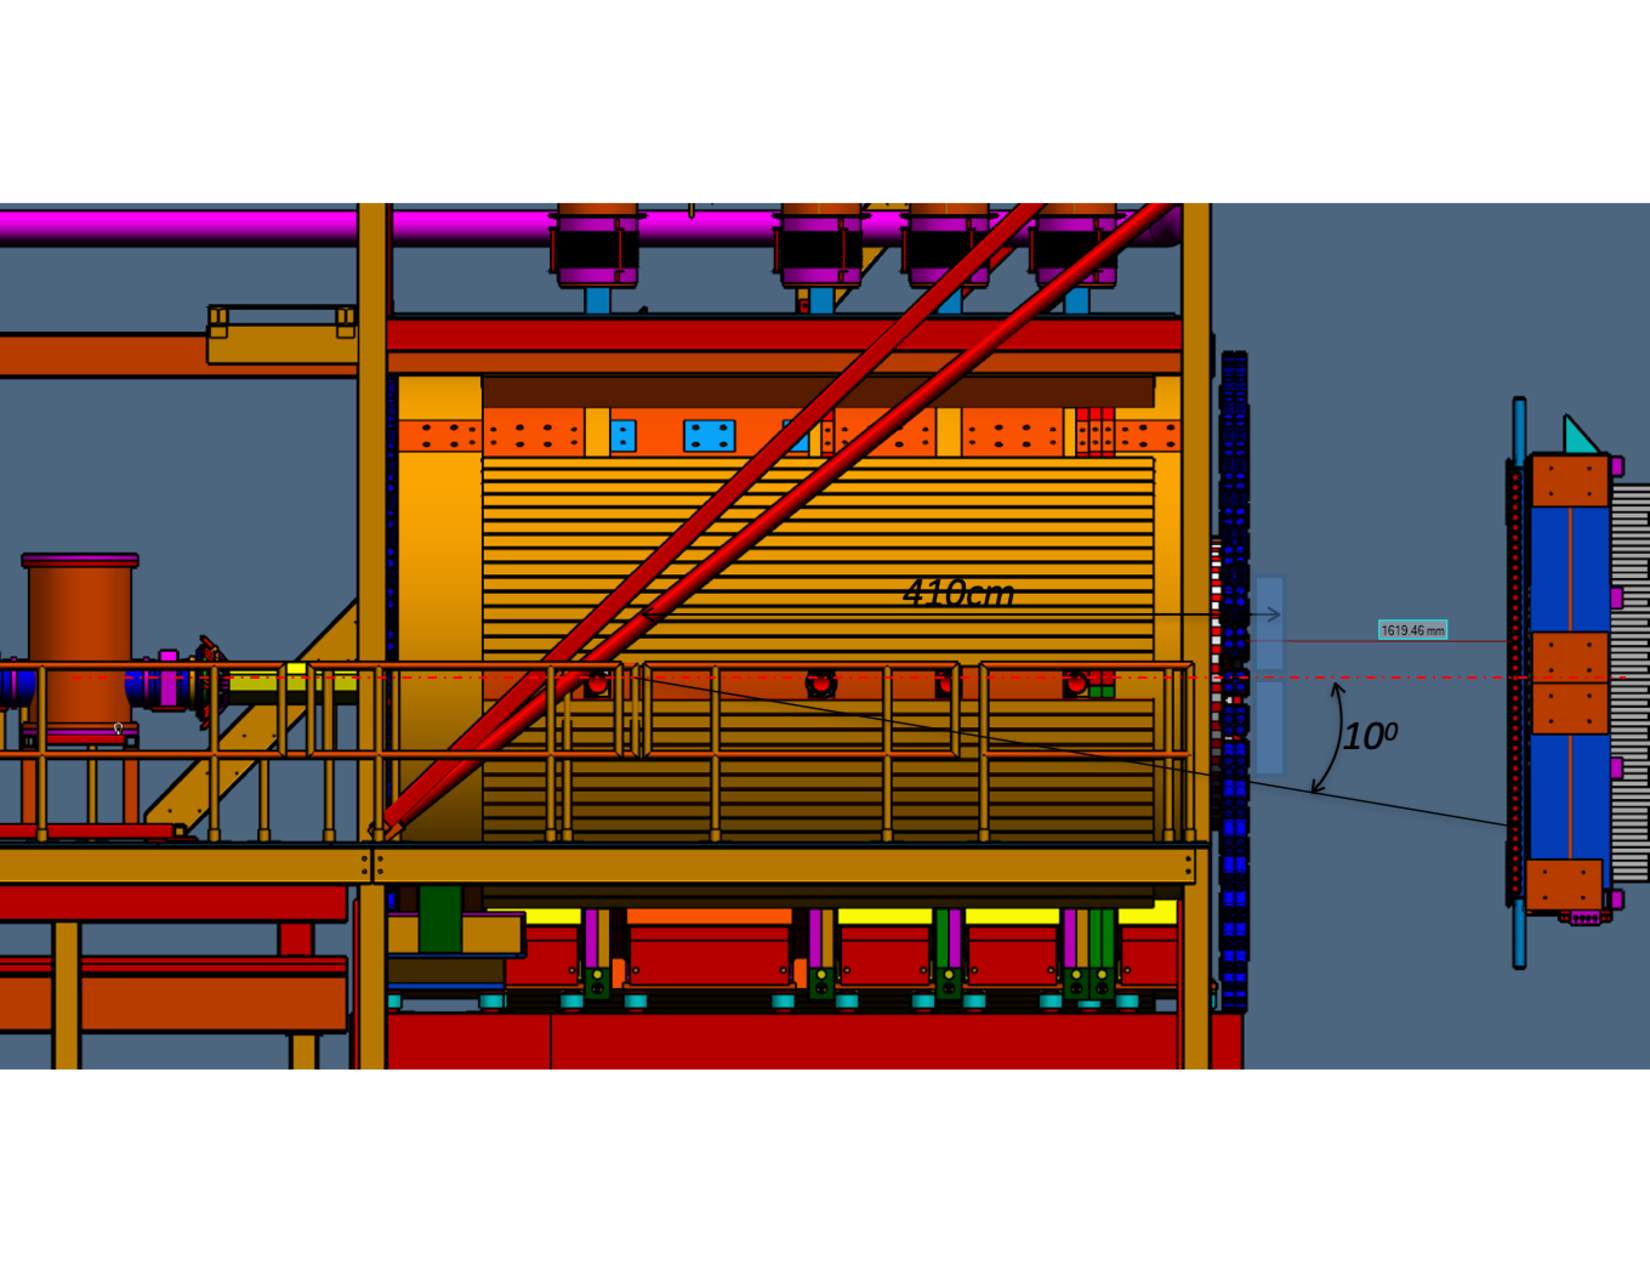
\includegraphics[width=0.80\textwidth]{./fig/GEM_TRD_side.pdf}
  \caption{
Side view showing the approximate position of the proposed GEM-TRD detector
(light blue boxes), at $410$~cm downstream of the target,
covering $86$\% of the forward GlueX acceptance of $\sim 10^\circ$ 
polar angle.
The DIRC detector not in the plot.
}
  \label{fig:side_view}
\end{figure}
\begin{figure}[]
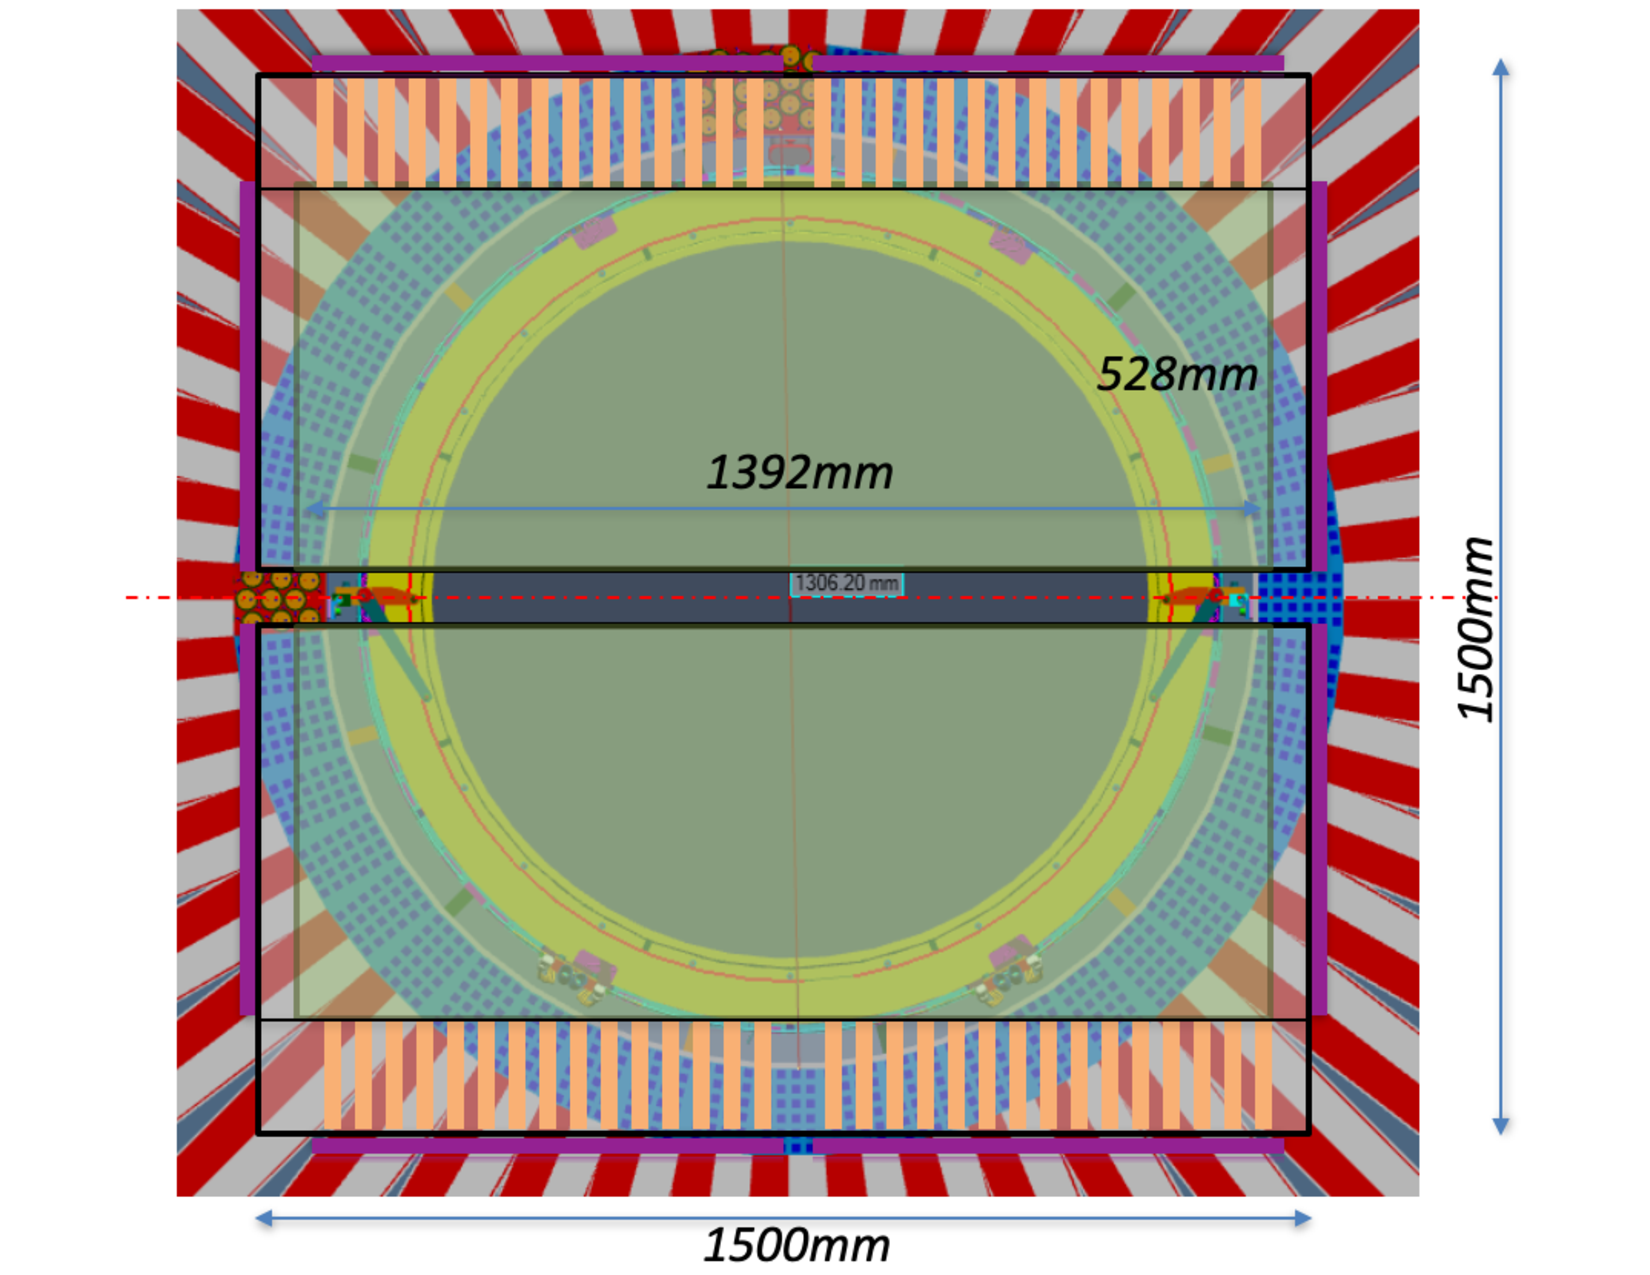
\includegraphics[width=0.80\textwidth]{./fig/GEM_TRD_full.pdf}
  \caption{
Front view of the GEM-TRD detector placed at the face of the solenoid
magnet. It consists of two separate chambers with $1392 \times 528$~mm$^2$
sensitive area. All the frames holding the front-end electronics
(purple thick lines) 
of sizes $\sim 1500 \times 1500$~mm$^2$
are outside of the GlueX forward acceptance.
}
  \label{fig:front_view}
\end{figure}

The detector has a radiator layer $15$~cm thick, followed 
by a $2$~cm drift volume, and a GEM stage combined with a readout board.
The principle of operation is illustrated in Fig.\ref{fig:principle}.
The Transition Radiation (TR) photons in the $keV$ region produced by the 
electrons in the radiator are absorbed by the Xe gas mixture in the drift volume
emitting electrons that drift to and are amplified by the GEM. 
The signals are readout from  X- and Y-strips on the readout board.
The horizontal strips are separated in the middle and readout 
from the left and right side of the chambers (Fig. \ref{fig:front_view}).
The strip pitch is $1$~mm, resulting in $2,448$ electronic channels
per chamber, or $4,896$ in total.
The signals are amplified on-board and then digitized with flash ADCs.
We assume using the same  electronics as for the GlueX drift chambers: 
GASII \cite{GASII} preamps and flashADC-125 \cite{fADC125},
however alternative better and cheaper options will be discussed bellow.
Thus we record the energy deposition along the track 
(measured by the drift time)
that has different profile for the TR photons
absorbed predominately at the entrance, and the track ionization 
that has uniform distribution, see Fig.\ref{fig:profile}. 
At the same time such detector works as a Time Projection Chamber,
allowing to reconstruct the track segment within the drift volume.

\begin{figure}[h]
  \begin{subfigure}[b]{0.40\textwidth}
    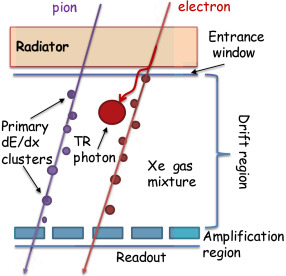
\includegraphics[width=\textwidth]{./fig/GEM_TRD_principle.jpg}
    \caption{GEM-TRD principle}
    \label{fig:principle}
  \end{subfigure}
  %
  \begin{subfigure}[b]{0.49\textwidth}
    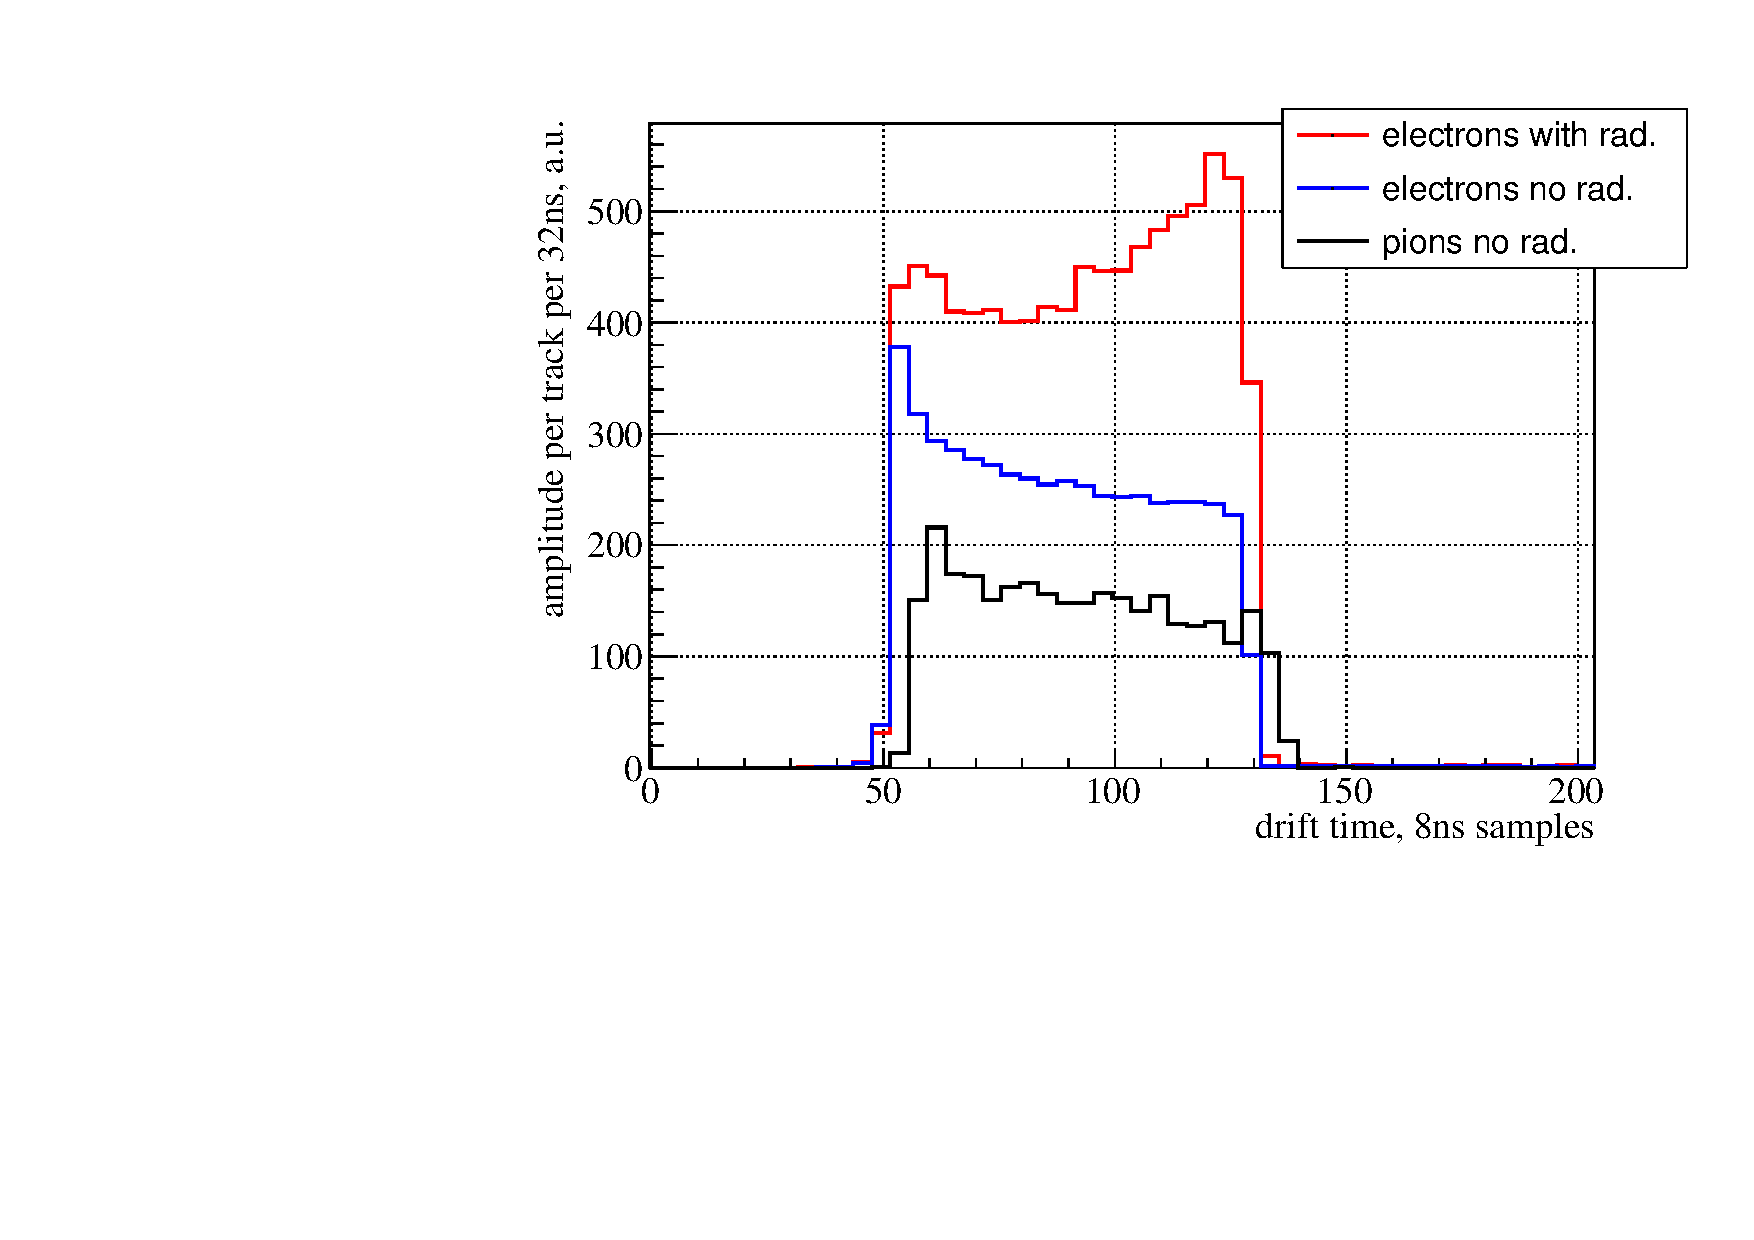
\includegraphics[width=\textwidth]{./fig/GEMTRD_piel_ampl_vs_t_left-2142.pdf}
    \caption{Amplitude profiles for electrons with and without radiator and pions;
data from studies with small prototypes}
    \label{fig:profile}
  \end{subfigure}
  \caption{
}
  \label{fig:BH_pove_pi}
\end{figure}

\begin{table}[h!]
\begin{ruledtabular}
\begin{tabular}{lcc}
\textrm{parameter}&
\textrm{value}&
\textrm{comment}\\
\colrule
sensitive area & $2 \times (1392 \times 528$~mm$^2)$ & two separate chambers\\
frame-free area & $1500 \times 1500~$mm$^2$ & except some minimal support \\
distance from the target & $4100$~mm & \\
forward acceptance coverage & $86$\% & for $e^+e^-$ invariant mass $>1.2$~GeV \\
radiator thickness & $150$~mm & \\
drift volume thickness & $20$~mm & \\
total detector thickness & $<4$\% R.L. & \\
drift field & $1.5$~kV/cm & \\
gas mixture & Xe/CO$_2$ $90/10$ & \\
maximum drift time & $800$~ns & \\
gas amplification & $\sim 5.10^4$ & \\
strip types & X and Y & on the same layer with capacitive coupling \\
strip pitch & $1$~mm & \\
readout channels & $4,896$ & $2,448$ per chamber \\
GASII pre-amps (24 channels) & $204$ & $102$ per chamber \\
GASII amplification & $2.4$ mV/fC & \\
flashADC-125 (72 channels) & $68$ & $34$ per chamber \\ 
VXS crates & 5 & \\
\end{tabular}
\end{ruledtabular}
\caption{
Main parameters of the GEM-TRD detector.
\label{tab:tech}
}
\end{table}
The main parameters of the GEM-TRD detector are given in Table \ref{tab:tech}.
They are based on tests with small prototypes ($10\times10$~cm$^2$)
done during the past several years, as discussed in the next section,
and are preliminary.
Further optimization of the detector will be done with a large-scale prototype
that will be built and tested during the 2022 and 2023 running periods.

\newpage
\section{Physics objectives}

The best approach to extract the absolute $J/\psi $ cross-sections is
to use the BH process for normalization using the formula \cite{prl_gluex}:
\begin{eqnarray}
\begin{array}{l}
\sigma = \frac{N_{J/\psi }}{N_{BH}}~\frac{\sigma_{BH}}{BR_{J/\psi}}~ \frac{\varepsilon_{BH}}{\varepsilon_{J/\psi }}\; ,
\label{eq:xsec}
\end{array}
\end{eqnarray}
where only the relative efficiency, $\varepsilon_{BH}/\varepsilon_{J/\psi }$,
of the $J/\psi $ and BH processes enters;
here $N_{BH}$ and $N_{J/\psi }$ are the yields of the corresponding processes,
$\sigma_{BH}$ -- the calculated BH cross-section, and $BR_{J/\psi}$ -- the
branching ratio of the $J/\psi \to e^+e^-$ decay.

\begin{figure}[]
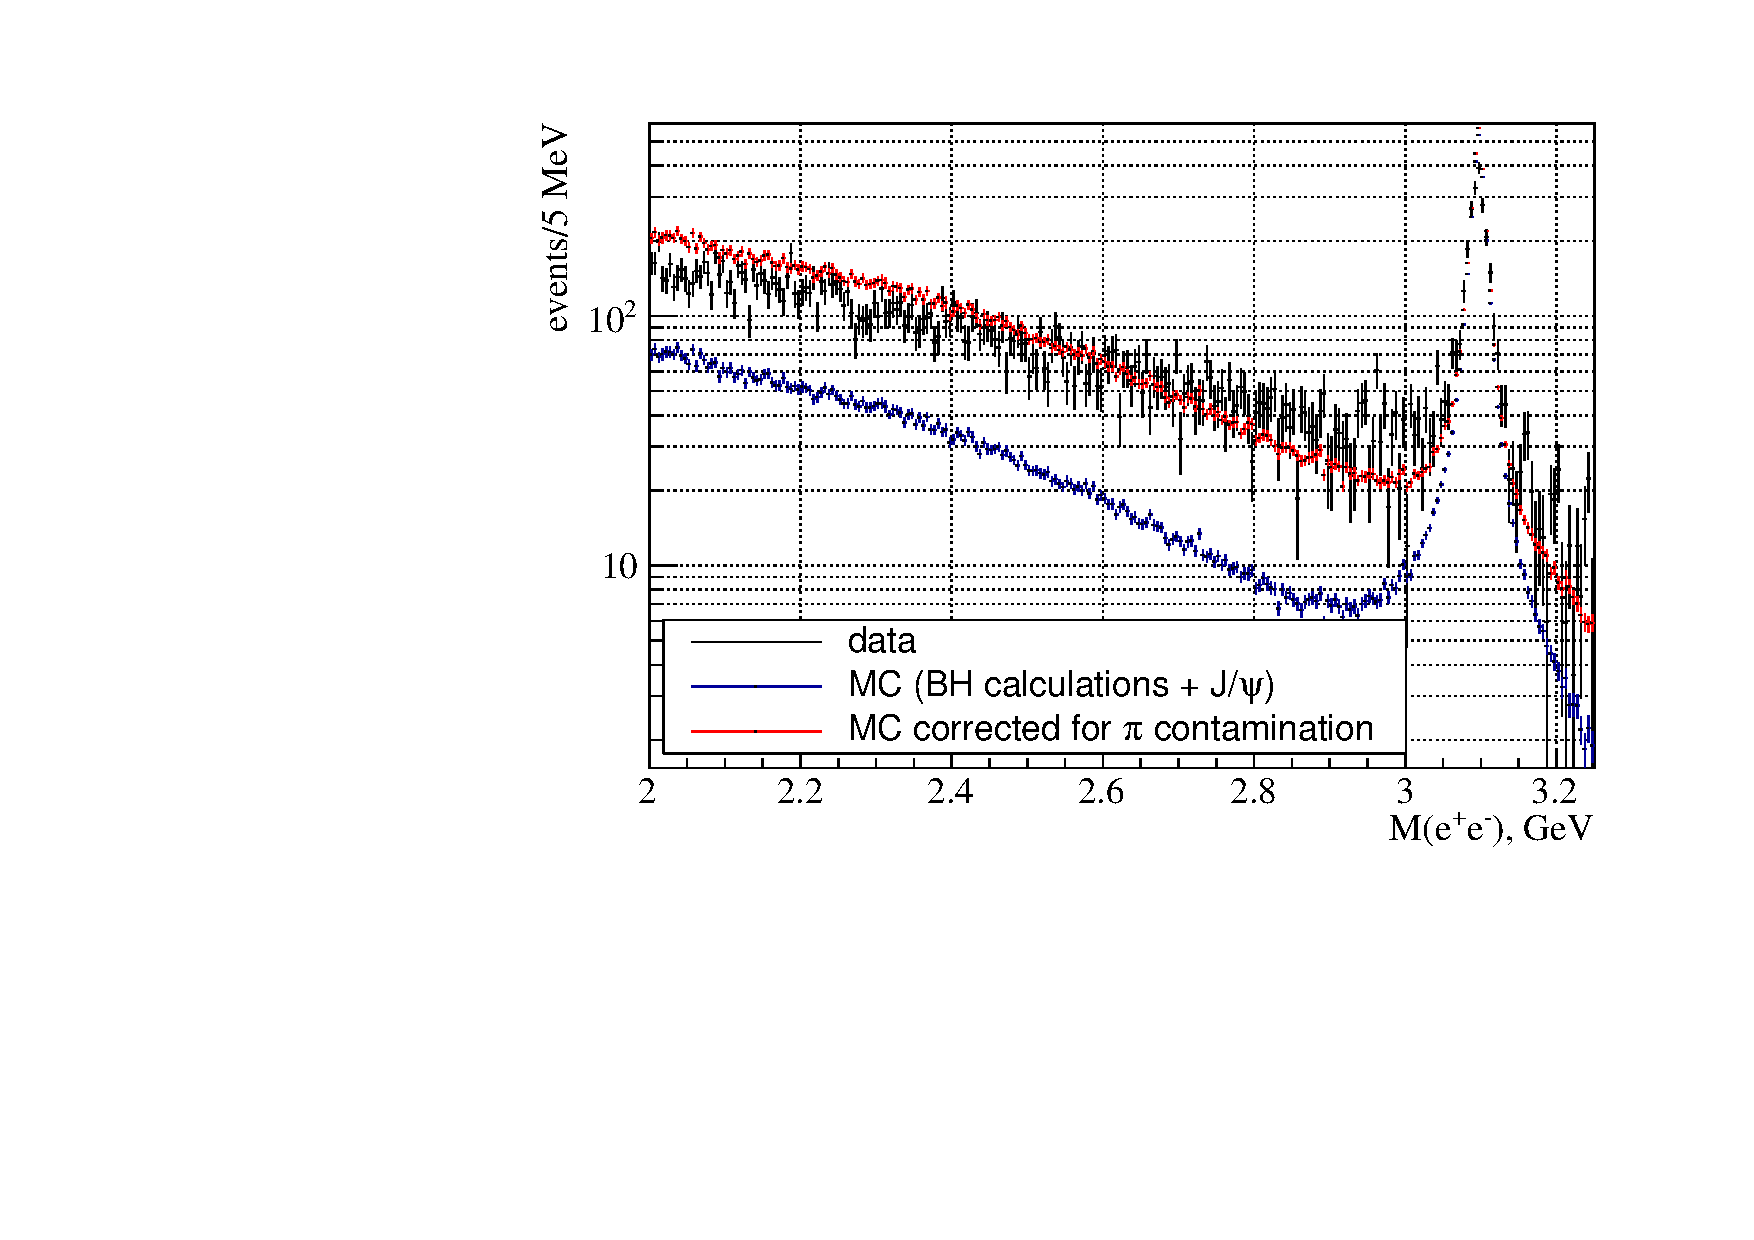
\includegraphics[width=0.80\textwidth]{./fig/GEM_TRD_minv_data_vs_MC.pdf}
  \caption{
The $e^+e^-$ invariant mass spectrum from data compared to 
Monte Carlo simulations that use absolute BH calculations
(as well as the $J/\psi $ photoproduction normalized to the data)
and their modification that adds the pion background (see text).
}
  \label{fig:minv}
\end{figure}
Fig.\ref{fig:minv} illustrates the problem with the pion background
in the GlueX detector.
It shows the $e^+e^-$ invariant mass spectrum from the data (black),
compared to simulations that include absolute calculations of the 
BH process \cite{Berger,Rafo,Jones} in the continuum 
and the $J/\psi $ peak normalized to the data (blue). 
For this plot we apply all the selections as explained in \cite{prl_gluex}.
Most importantly, $3\sigma $ cuts are applied 
around the peaks in the $p/E$ distributions
($p$ is the momentum and $E$ the energy deposited in the corresponding
calorimeter, BCAL and FCAL)
for both, the electron and the positron candidates. 
Additional selection is applied  on the signal from 
the first layer of BCAL, that works as a pre-shower.
As we register all the final state particles and have very good 
precision for the beam photon energy,
we can apply a Kinematic Fit (KF) that constrains the four momenta
and the vertex position of the final state particles.
The KF reduces significantly the background, as discussed below.

Thus, after all selections applied, the pion background is of the same order
as the signal and, therefore, we have to use some statistical procedures
to estimate the background and extract the BH yields.
The result of such procedure is shown on the same plot --
the red points in Fig.\ref{fig:minv} correspond to the simulations (blue) 
to which the pion background is added using 
the signal-to-background ratios in Figs.\ref{fig:sb_FCAL},\ref{fig:sb_BCAL}. 
Examples of $p/E$ fits used to estimate these ratios from the data are given in the Appendix.
\begin{figure}[h]
  \begin{subfigure}[b]{0.49\textwidth}
    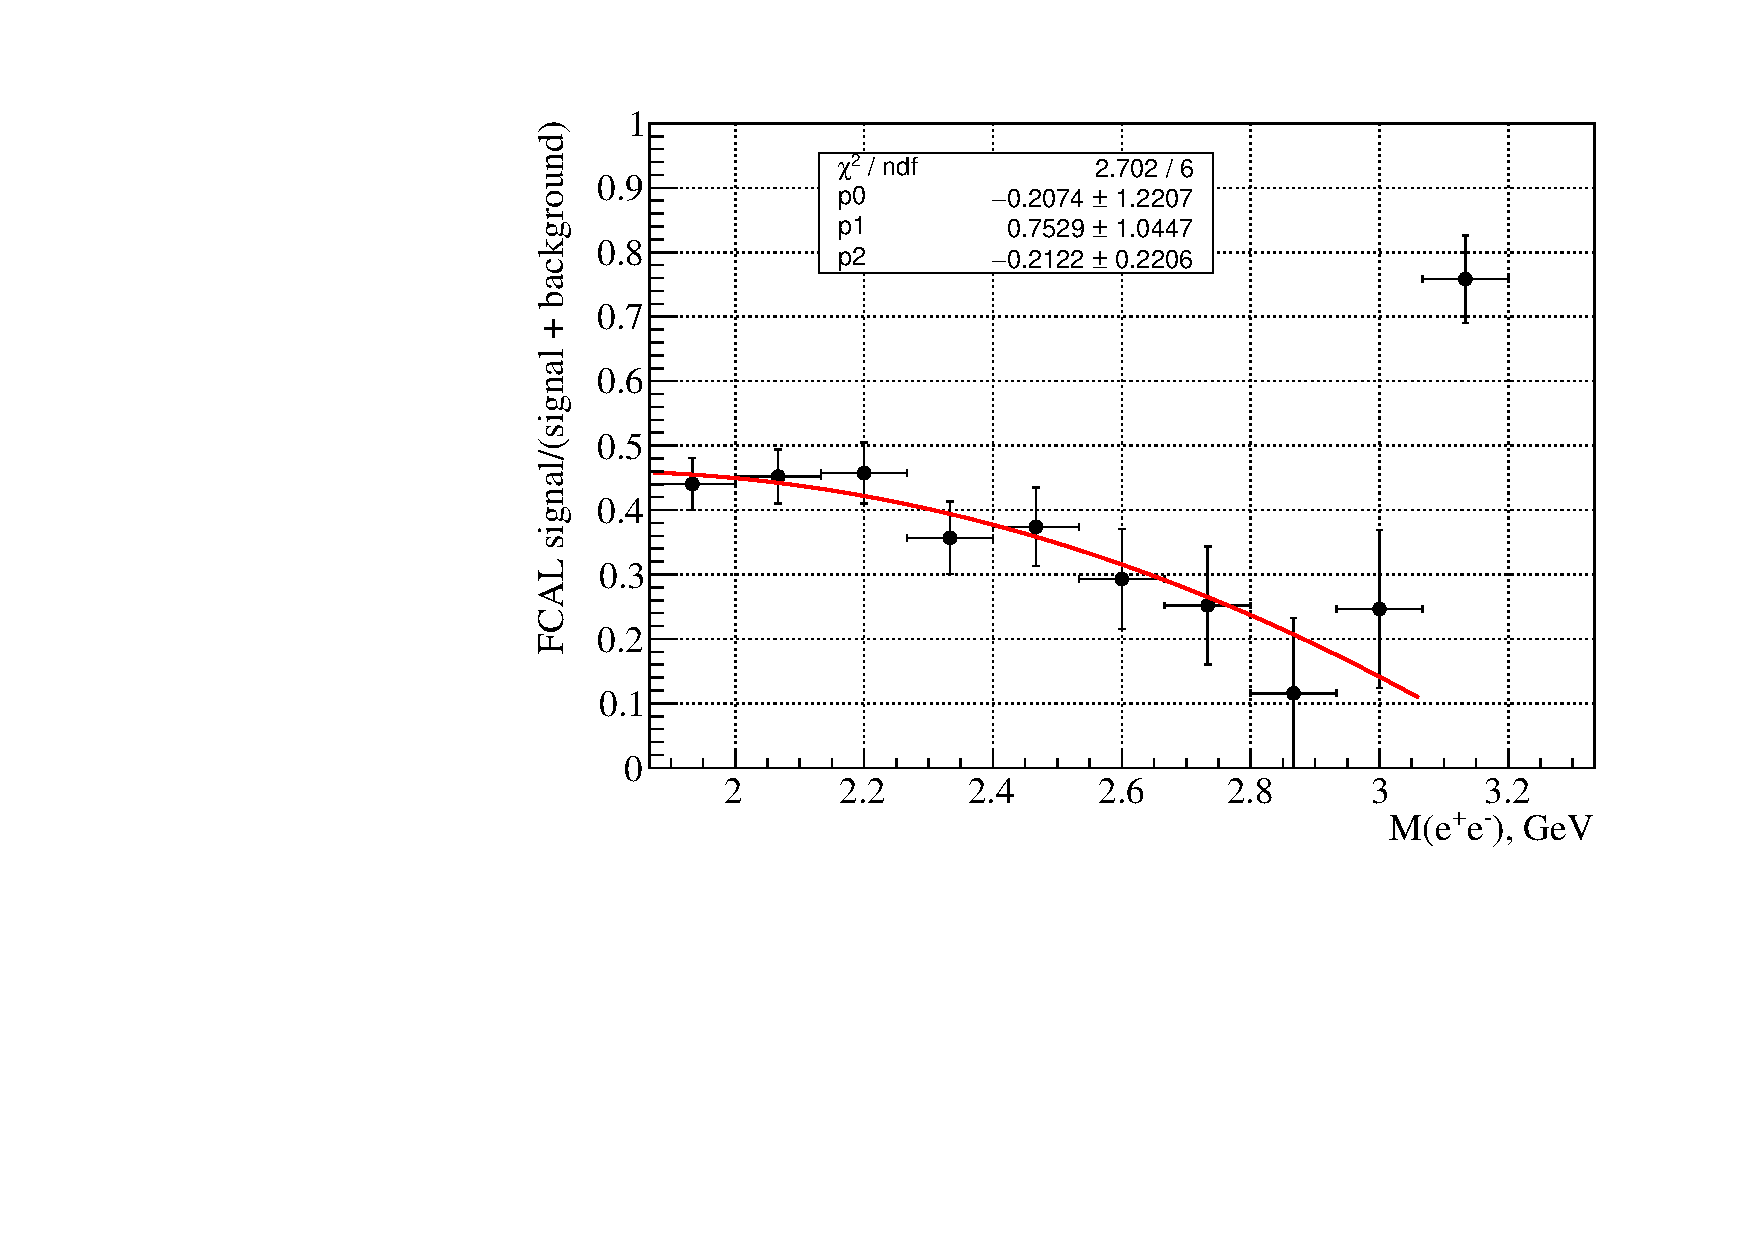
\includegraphics[width=\textwidth]{./fig/GEM_TRD_sb_FCAL.pdf}
    \caption{ 
FCAL
}
    \label{fig:sb_FCAL}
  \end{subfigure}
  %
  \begin{subfigure}[b]{0.49\textwidth}
    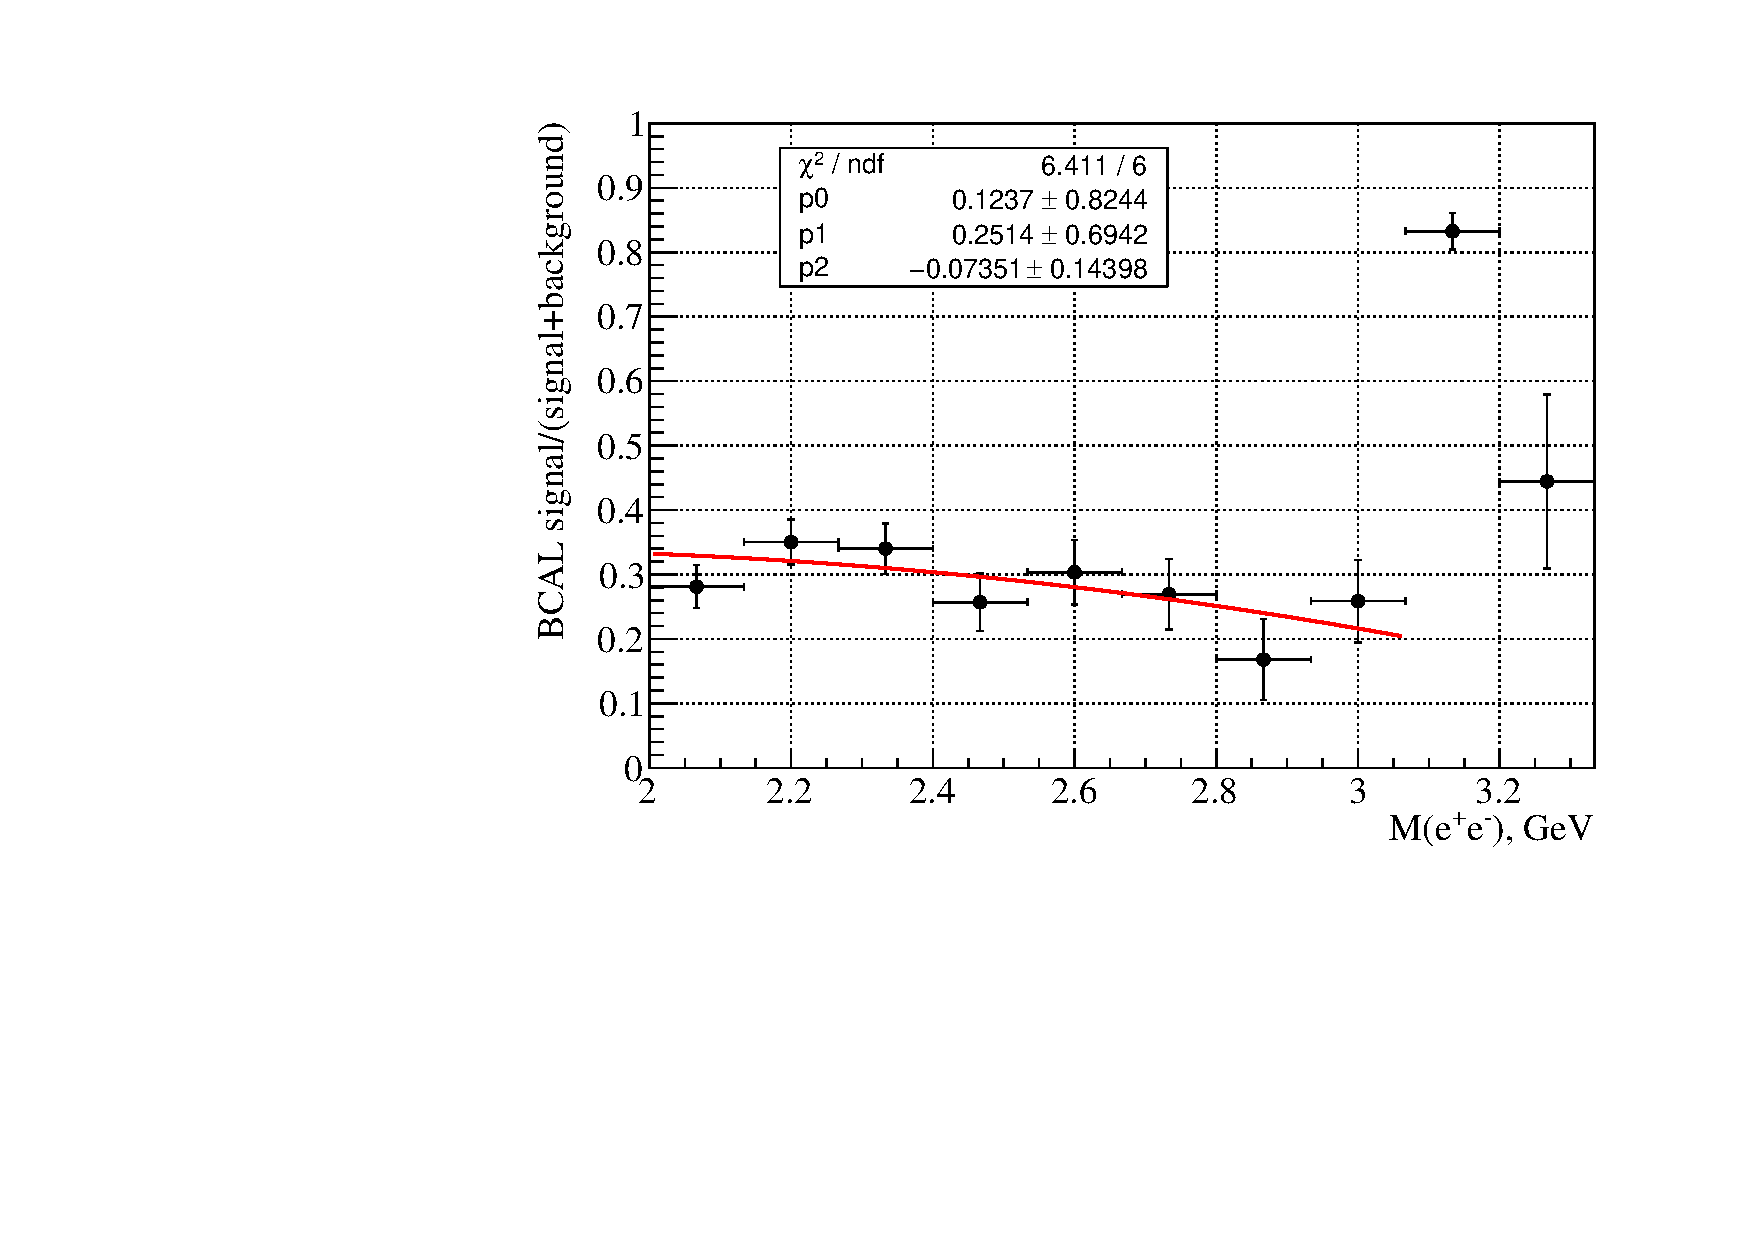
\includegraphics[width=\textwidth]{./fig/GEM_TRD_sb_BCAL.pdf}
    \caption{ 
BCAL
}
    \label{fig:sb_BCAL}
  \end{subfigure}
  \caption{
The signal to (signal+background) ratio for the two calorimeters as function
of the  $e^+e^-$ invariant mass fitted with a polynomial.
}
  \label{fig:sb}
\end{figure}

In Fig.\ref{fig:minv_BFCAL} we plot the  $e^+e^-$ mass spectra for two cases,
when at least one lepton goes forward and when both leptons are registered 
in the BCAL.
The pion background is much more significant in the forward direction,
where the GEM-TRD will be installed.
This can be explained by the fact that background reactions like 
$\gamma p \to \Delta \pi \to p \pi \pi$ ($\Delta $ can be any other nuclonic resonance)
will produce predominately one forward pion and one backward 
coming from the target excitation.
\begin{figure}[]
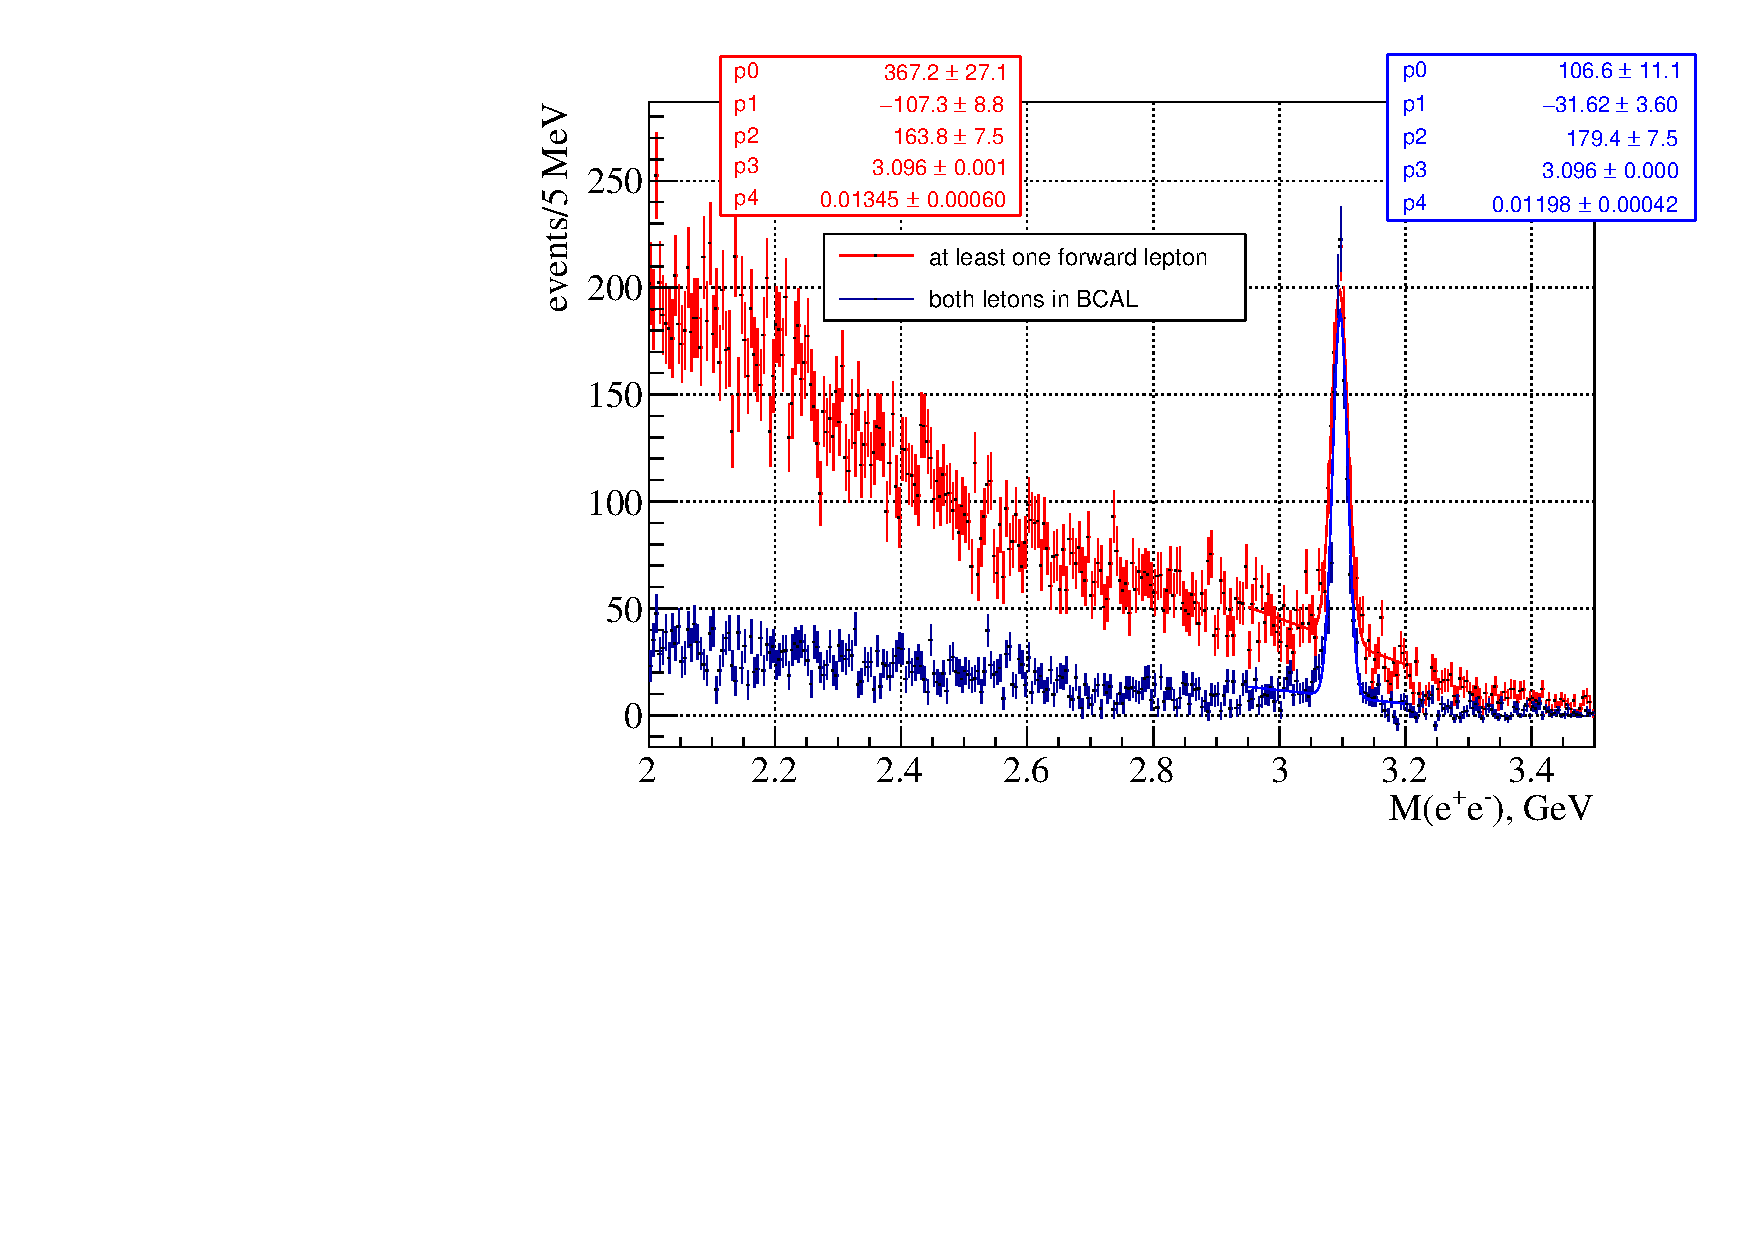
\includegraphics[width=0.80\textwidth]{./fig/GEM_TRD_Minv_one_in_FCAL_comp.pdf}
  \caption{
The $e^+e^-$ invariant mass spectrum from data  
in case of at least lepton goes in the forward direction,
and when both leptons are registered in BCAL.
The background below the $J/\psi $ peak $\pm 3\sigma $ in forward direction is $65$\%.
}
  \label{fig:minv_BFCAL}
\end{figure}


\subsection{Improving the systematics of the $J/\psi $ photoproduction
using GEM-TRD}

\subsubsection{Pion rejection efficiency}
The simulation of the calorimeter response to pions is not perfect.
Thus, the selections applied to data and simulations may have
different efficiencies. 
This is seen when comparing the $p/E$ distributions from data and MC 
(see Appendix).
At the same time, the $p/E$ cuts are the most important in rejecting the pions.
The fitting procedures to extract the $e^+e^-$ yields are very sensitive
to these selections and suffer from instability, 
especially for FCAL due to the steep background.
One can try to do effective corrections to the simulations based on the data,
however, due to the momentum and angular dependence of these correction,
this is not possible in practice.
Therefore, so far, we were not able to attribute any systematic error
related to the pion rejection efficiency.
The best solution would be to use the GEM-TRD in front of the FCAL to create
a clean sample of electrons and measure the FCAL rejection efficiency.
For that we don't need the whole acceptance of the GlueX detector
and propose to do such measurements, first, with one chamber only 
-- see the timeline of the proposal in Sec.\ref{sec:time}.
Then, the results of these measurements can be used for the whole data set
to improve the simulations and assign a realistic systematic error.

\subsubsection{The efficiency of the Kinematic Fit}

The Kinematic Fit (KF) cuts more than $50$\% of the final state particle candidates,
therefore potentially it is a significant source of systematic errors.
However, it is needed because it improves the $e^+e^-$ mass resolution
and reduces the background significantly, especially in the forward direction.
As for the mass resolution, 
there is an alternative of using the measured electron/positron
momenta and angles. 
Fig.\ref{fig:mrec} shows the $e^+e^-$ mass spectrum as measured by
the missing mass off the recoil proton with and without the KF,
in the case of at least one lepton in the forward direction.
The mass resolution is as good as the standard reconstruction,
however the background without
the KF is significant and doesn't allow to extract the cross sections
reliably, as the fluctuation of the background are similar in size 
to the $J/\psi $ peak.
Again, the use of the GEM-TRD would reduce the background to about $10$\%
allowing to do studies with and without the KF and measure its efficiency.
\begin{figure}[]
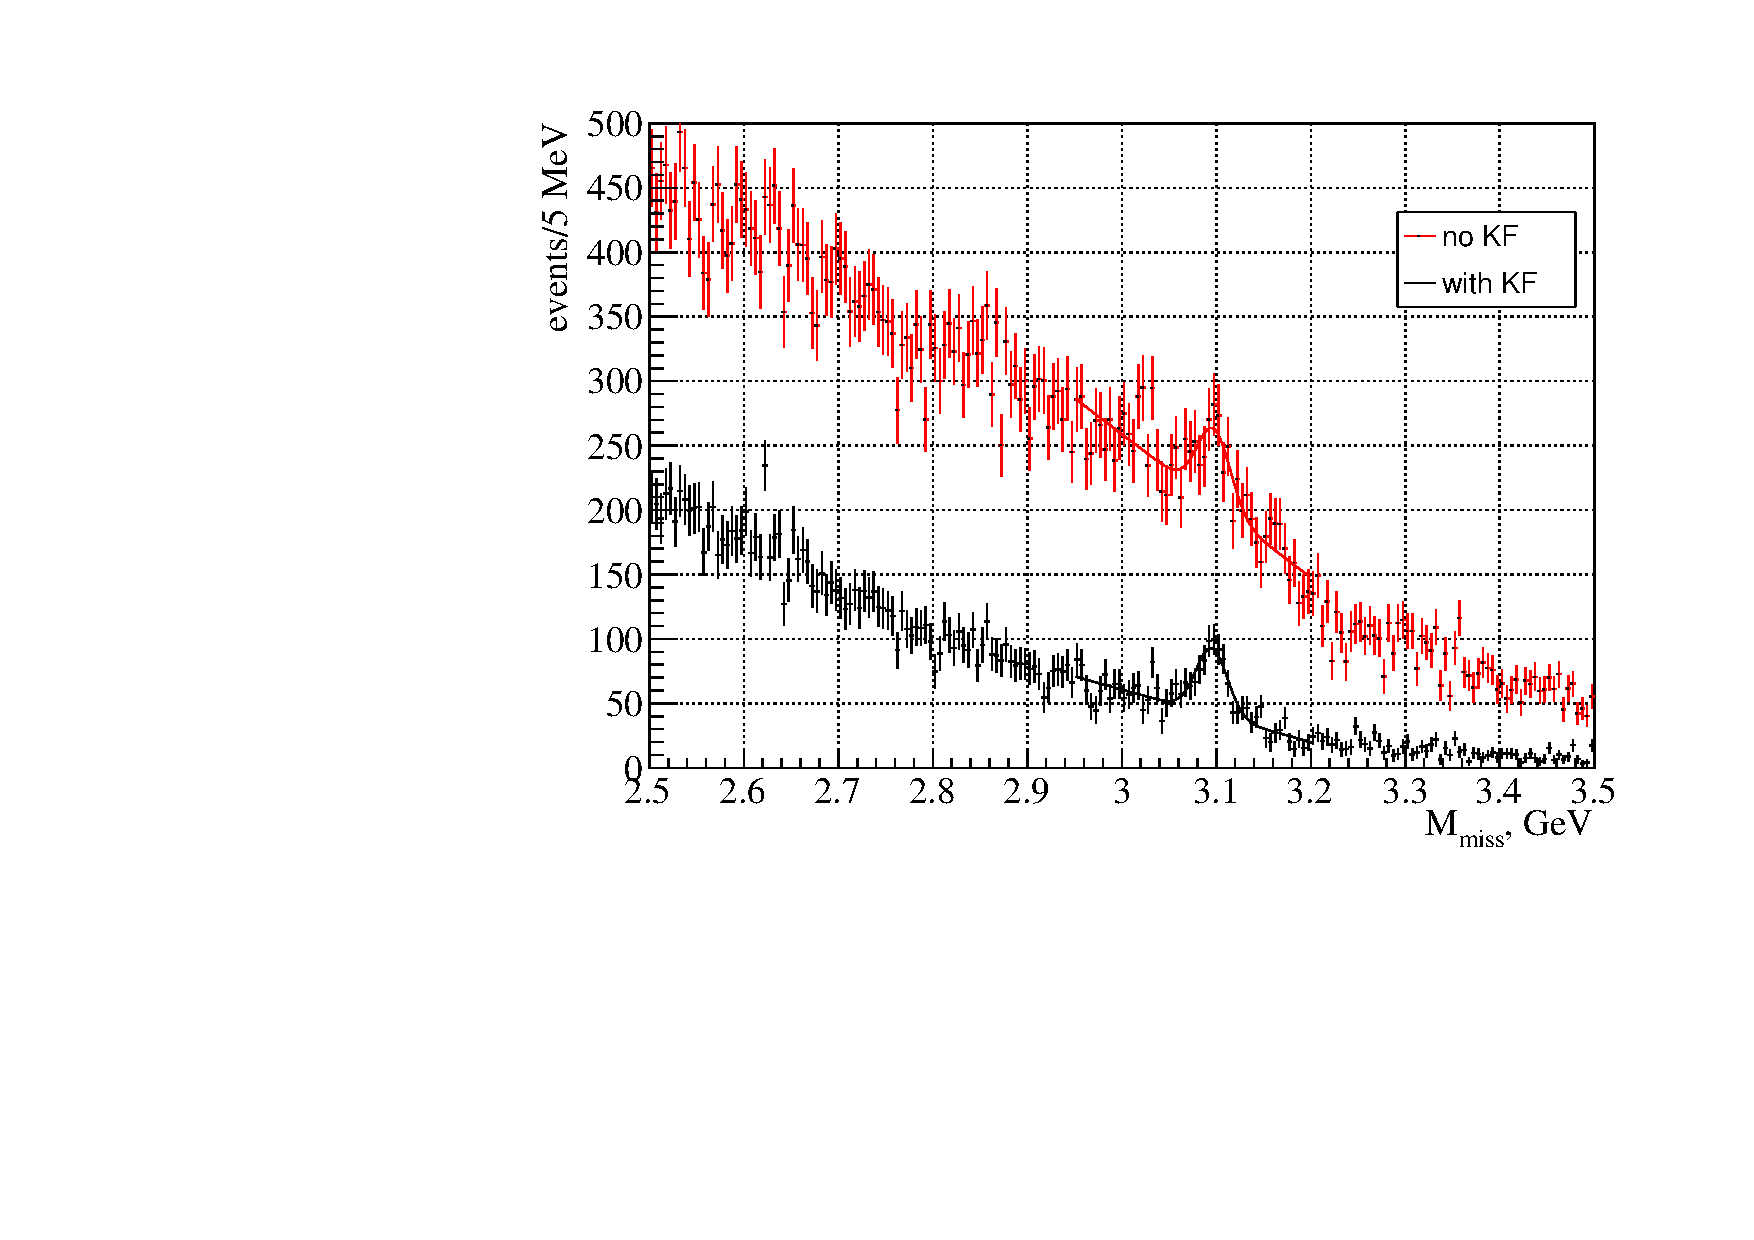
\includegraphics[width=0.80\textwidth]{./fig/GEM_TRD_Minv_no_with_KF.pdf}
  \caption{
The missing mass off the recoil proton from the data 
with and without Kinematic Fit (KF), with at least one forward lepton.
}
  \label{fig:mrec}
\end{figure}

\subsubsection{BH normalization}

Fig.\ref{fig:BH_Minv_data_MC} compares the measured
BH cross sections to the absolute calculations,
as function of the invariant mass.
\begin{figure}[h]
  \begin{subfigure}[b]{0.49\textwidth}
    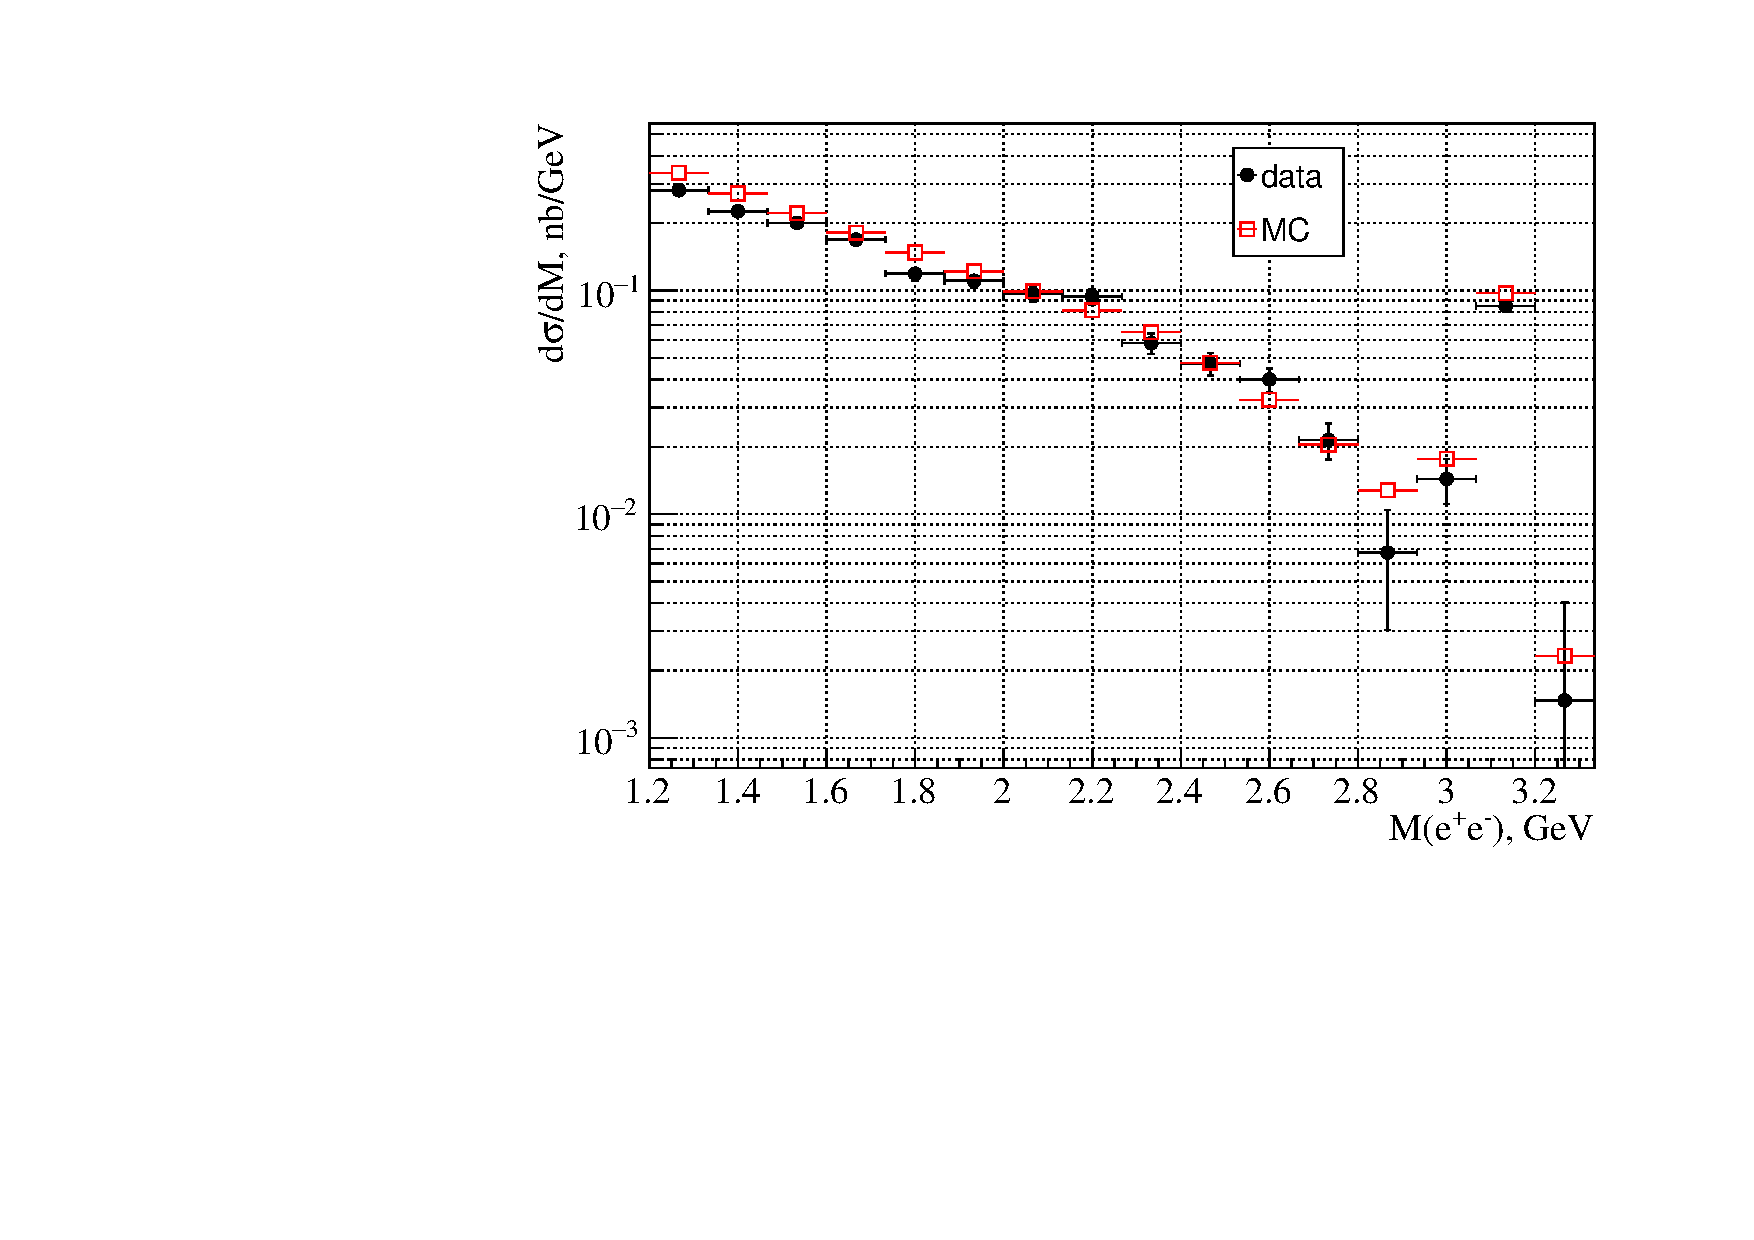
\includegraphics[width=\textwidth]{./fig/AN2_BH_Minv_comp.pdf}
    \caption{BH cross-sections from data and MC.}
    \label{fig:BH_Minv_comp}
  \end{subfigure}
  %
  \begin{subfigure}[b]{0.49\textwidth}
    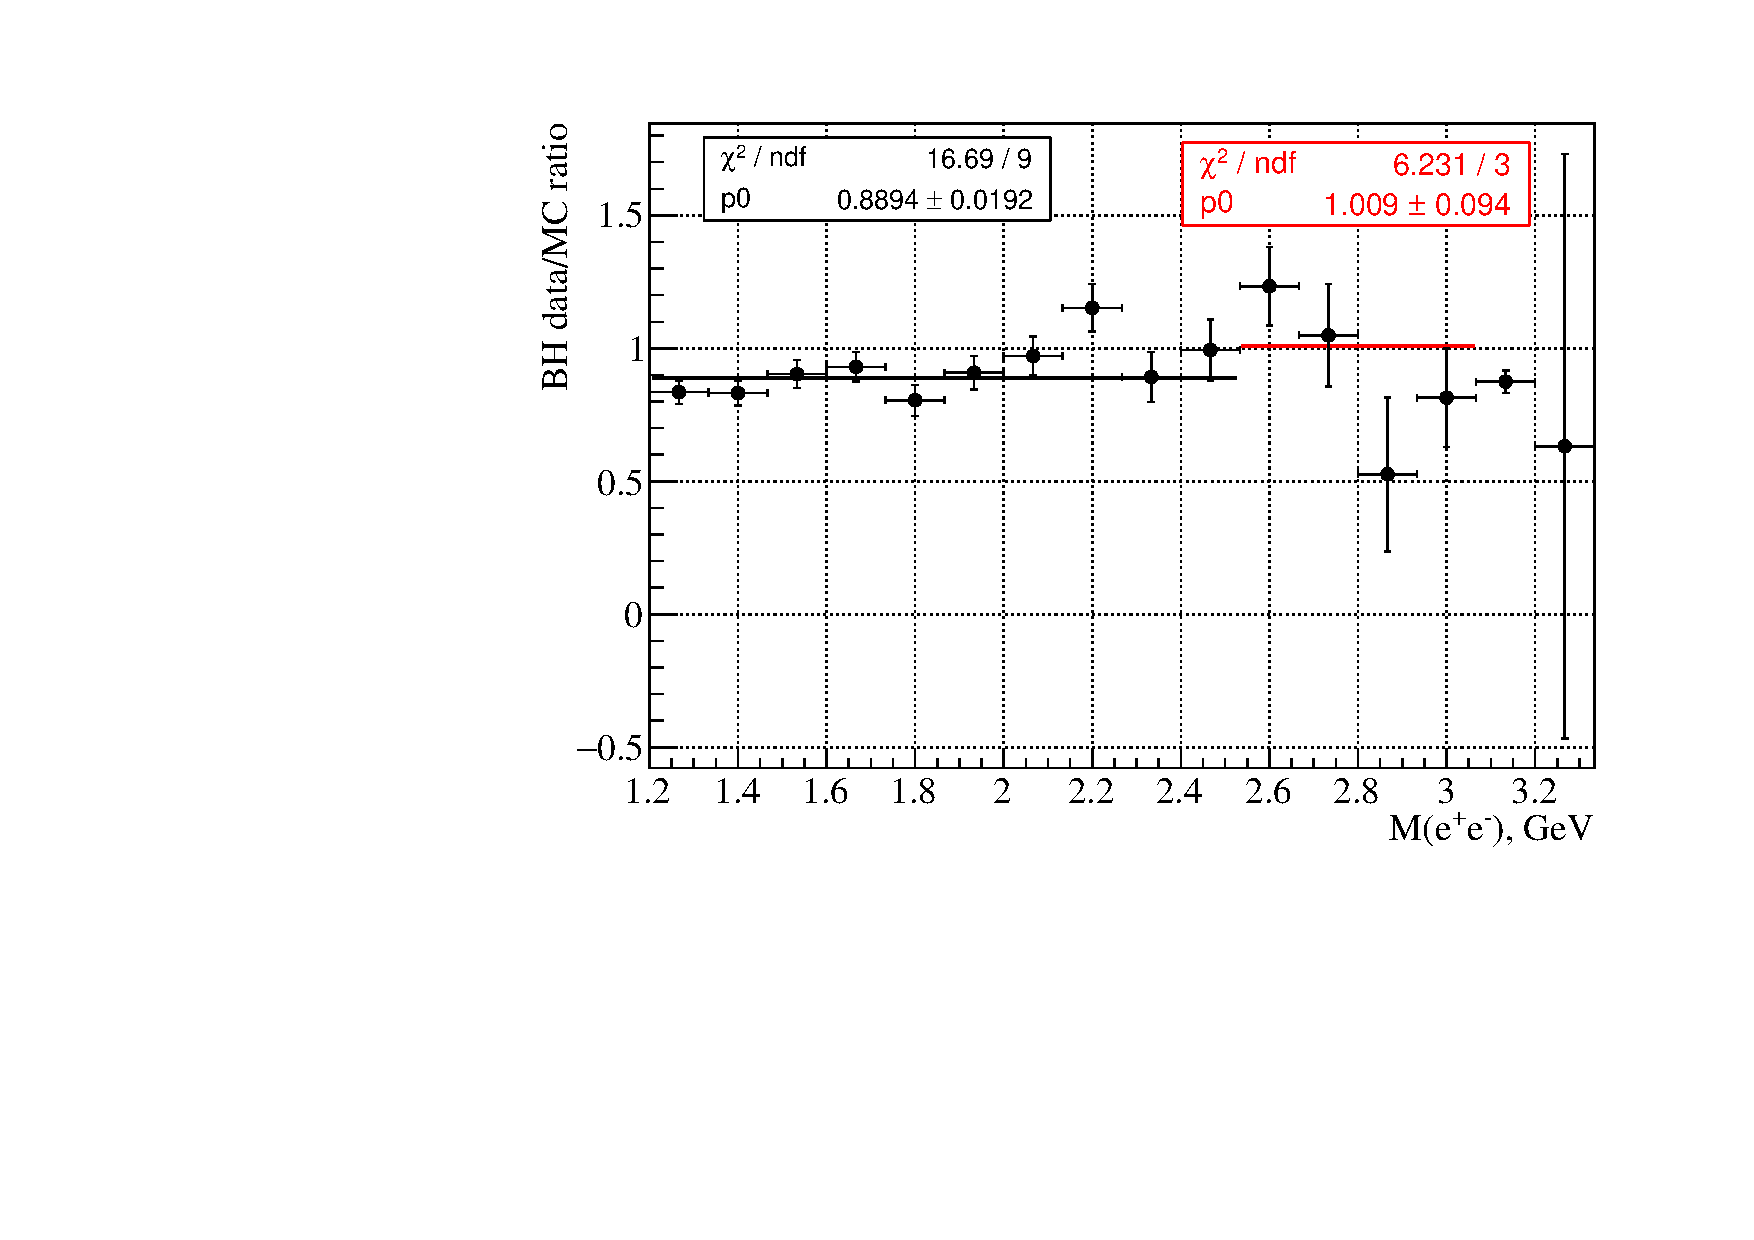
\includegraphics[width=\textwidth]{./fig/AN2_BH_Minv_ratio.pdf}
    \caption{BH data/MC ratio from Fig.\ref{fig:BH_Minv_comp} fitted with constants in two regions.}
    \label{fig:BH_Minv_ratio}
  \end{subfigure}
  \caption{
BH cross-section vs invariant mass: data vs MC.
}\label{fig:BH_Minv_data_MC}
\end{figure}
One can see from Fig.\ref{fig:BH_Minv_ratio} that the data/MC ratio 
is not constant and shows a tendency of increasing towards the $J/\psi $ peak,
however with a significant uncertainty.
Based on such studies we estimated \cite{prl_gluex} a contribution to the 
normalization uncertainty
of about $25$\%, which is the dominant contribution to the systematics.
We suspect that such data-MC inconsistency comes from the 
problems discussed in the previous subsections, the poor knowledge
of the pion rejection and the KF efficiencies. 
In addition, we found that the errors of the cross section
are dominated by the background fluctuations when fitting
the $p/E$ distributions (see Appendix). 
If we assume no pion background, the errors will be defined 
simply by the number of events, then our estimation of the 
normalization uncertainty would go down below $10$\%.


\subsection{Amplitude Analysis of the $J/\psi $ photoproduction and search
for the LHCb pentaquarks}

If the LHCb pentaquarks \cite{LHCb1,LHCb2} exist, they should be seen in the $s$-channel
of the $J/\psi $ photoproduction \cite{Kubarovsky,Karliner,Blin}.
The negative results coming from JLab \cite{prl_gluex}
mean that indeed, if such states exist, we need more precise tools
to identify them. 
Performing amplitude analysis over the whole kinematic space 
has the potential to uncover such states, or set much lower limits
on their existence.
The GlueX detector has acceptance in the full kinematic range
next to the threshold where the pentaquark region is, see Fig.\ref{fig:dsdt}.
However, the amplitude analysis requires knowledge of the amplitudes
of the contributing reactions, including the background which is significant
especially in forward direction, where it reaches $65$\% within 3$\sigma $ of
the $J/\psi $ peak, see Fig.\ref{fig:minv_BFCAL}.
The GEM-TRD will reduce the pion contamination for the $J/\psi $ events to about $5$\%
that will make the amplitude analysis much more reliable.

(expect contribution from Alex ... )

\begin{figure}[]
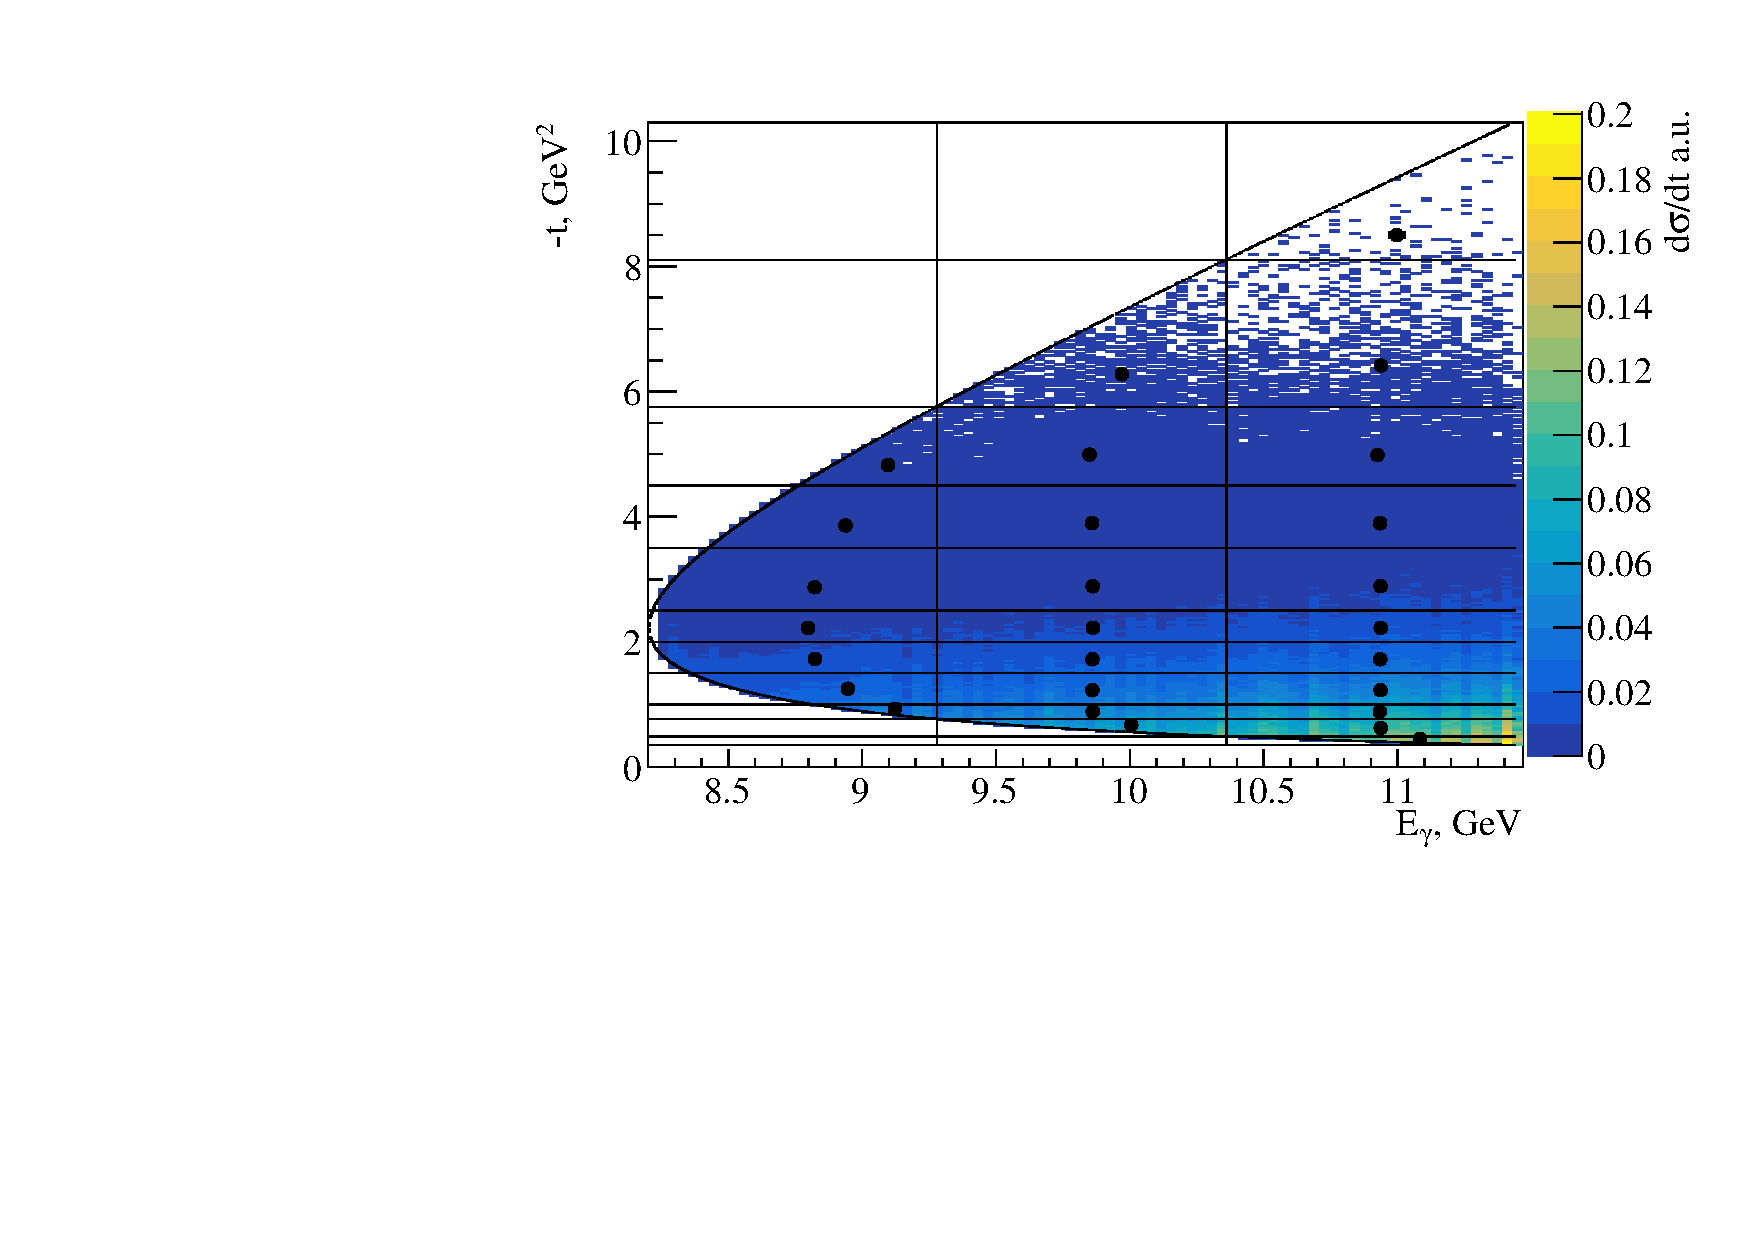
\includegraphics[width=0.80\textwidth]{./fig/AN4_to_theor1_TMC.pdf}
  \caption{
The coverage of the kinematic space of the 
$J/\psi $ photoproduction near threshold, with bins where GlueX
will provide measurements of the $2D$ differential cross section. 
Shown are results from simulations, just for illustration. 
}
  \label{fig:dsdt}
\end{figure}

\subsection{Other di-electron reactions to be studied with GlueX}

... TCS (including beam asymmetries?) ... expect contribution from Sean ... 

\subsection{Improving the tracking with the GEM-TRD}

... Lubomir will work on this ..

\newpage
\section{Studies with prototypes}
 
\begin{figure}[h]
  \begin{subfigure}[b]{0.49\textwidth}
    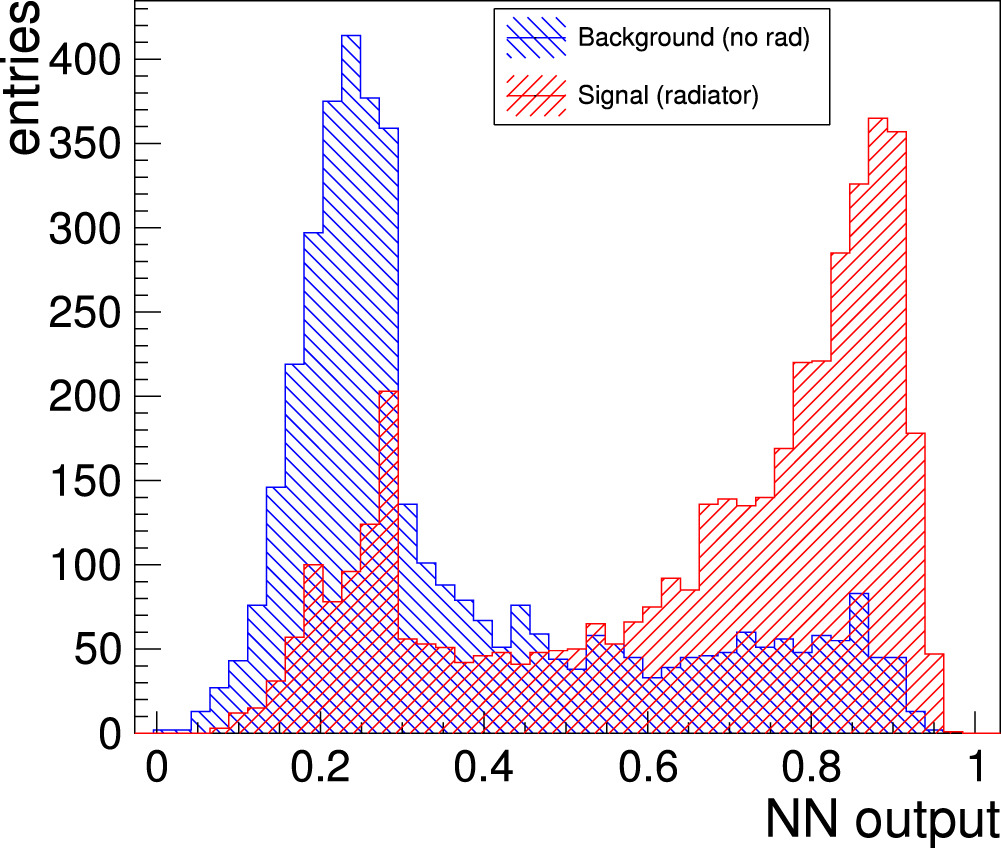
\includegraphics[width=\textwidth]{./fig/GEM_TRD_NNoutput.jpg}
    \caption{Neural Network (NN) output for electrons with and without 
radiator}
    \label{fig:NNout}
  \end{subfigure}
  %
  \begin{subfigure}[b]{0.40\textwidth}
    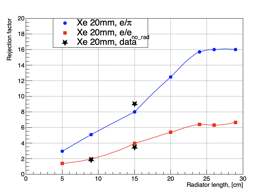
\includegraphics[width=\textwidth]{./fig/pion_rejection.png}
    \caption{Pion rejection factor from data (stars) 
and simulations from radiator/no radiator (red)
and electron/pion (blue) comparison;
data from studies with small prototypes}
    \label{fig:rejection}
  \end{subfigure}
  \caption{
}
  \label{fig:BH_pove_pi}
\end{figure}
Studies with small ($10 \times 10$cm$^2$) prototypes have been done
during 2018-2021.
They were performed both with electrons, at one of the Pair Spectrometer arms,
and with pions in the forward GlueX acceptance, downstream of the magnet
and in front of the DIRC detector.
Some results of these measurements were presented already in Sec.\ref{sec:detector},
showing the timing profile of the detector response for electrons with/without radiator
and for pions, Fig.\ref{fig:profile}.
Event-by-event analyses using neural network were done 
(Fig.\ref{fig:NNout}, Fig.\ref{fig:rejection}) 
demonstrating a factor of $\sim 4$ effect of the radiator with electrons,
and $\sim 10$ pion rejection factor, the later based on experiments with
electrons at pions done separately.

Such measurements proved the principle of using GEM technology for TR detectors.
At the same time they helped to specify the parameters of next, large-scale prototype.
This prototype will cover a quarter of the final detector (Fig.\ref{fig:proto}),
allowing to be used for real physics data taking.
It will be produced under a contract with UVA that already started.
We will use existing spare electronics to test it during 2022-2023.
\begin{figure}[]
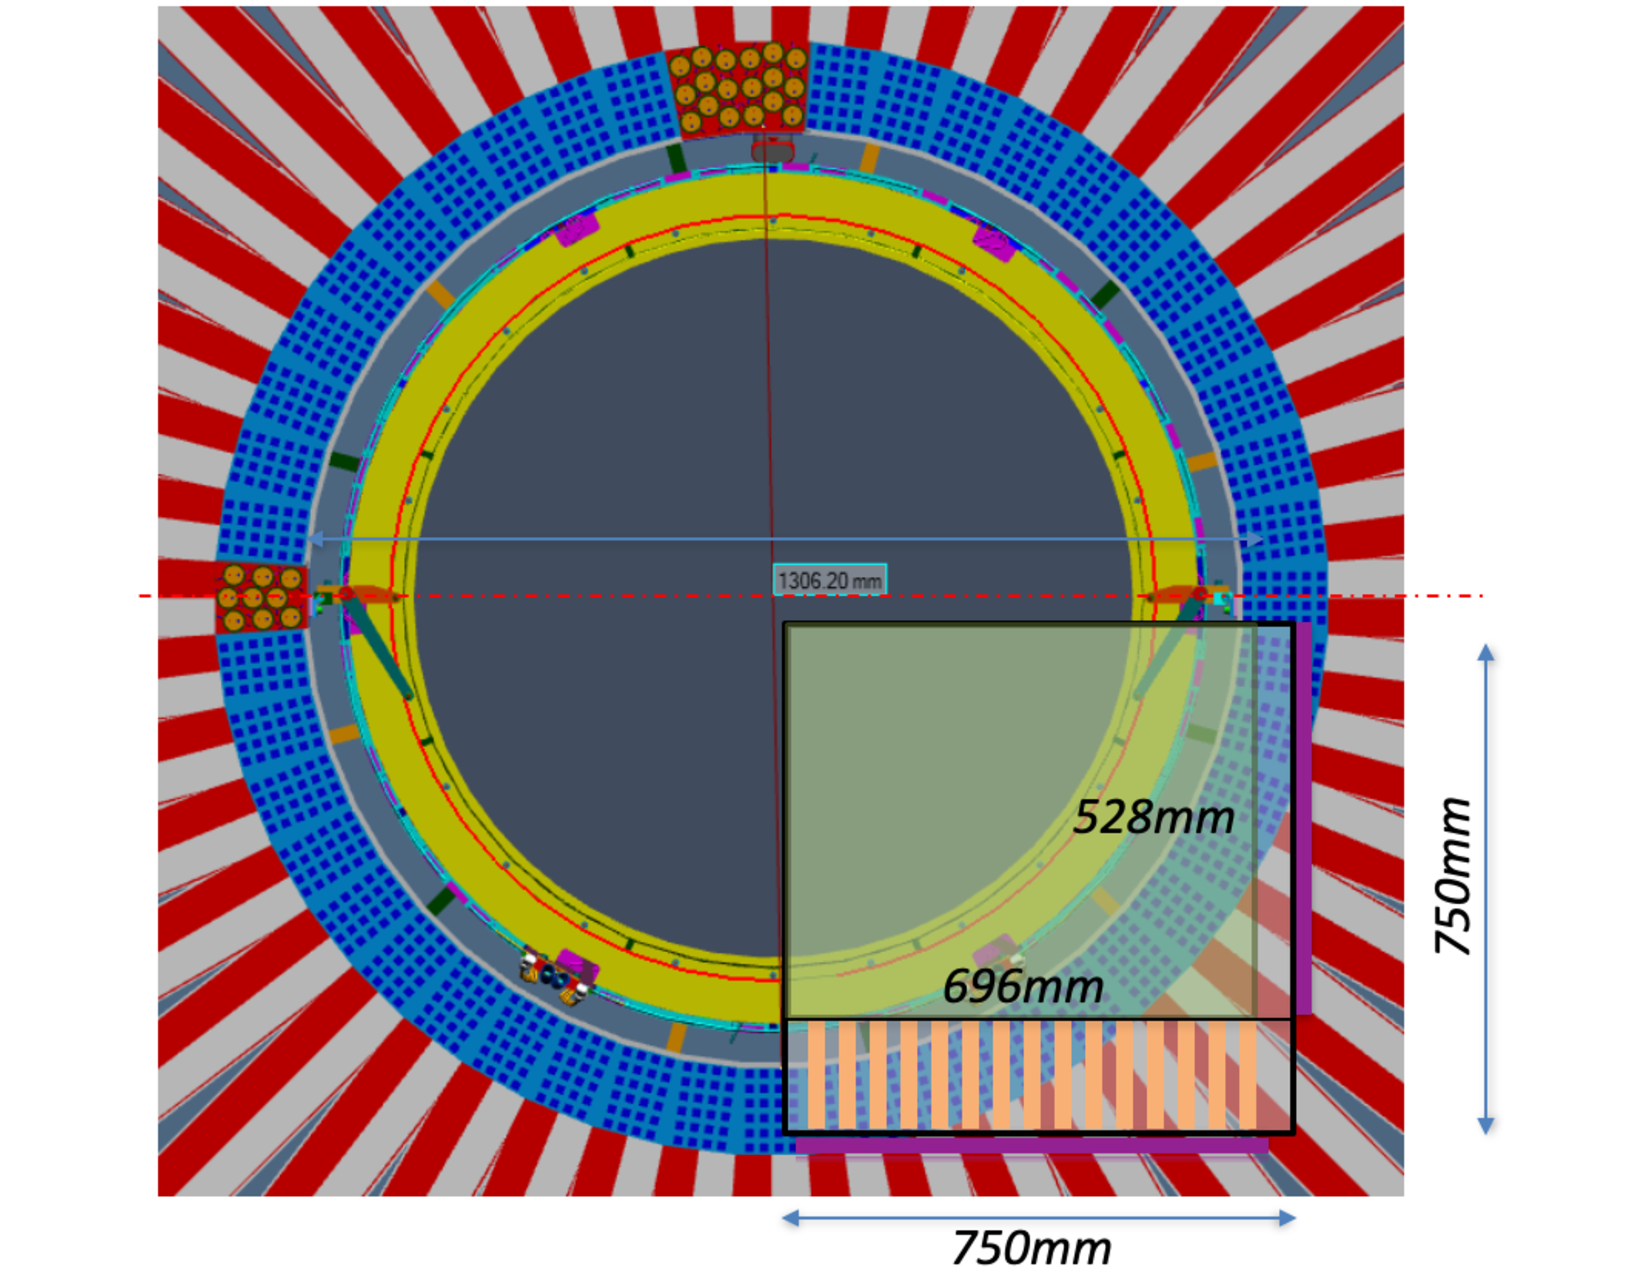
\includegraphics[width=0.80\textwidth]{./fig/GEM_TRD_prototype.pdf}
  \caption{
Front view of the GEM-TRD large-scale prototype
that has $696 \times 528$~mm$^2$ 
sensitive area. 
}
  \label{fig:proto}
\end{figure}


\section{Gas System Requirements}
The high price of the Xe gas requires system that recirculates
and purifies the gas mixture.
The principle diagram of such system is shown in Fig.\ref{fig:gas}.
\begin{figure}[]
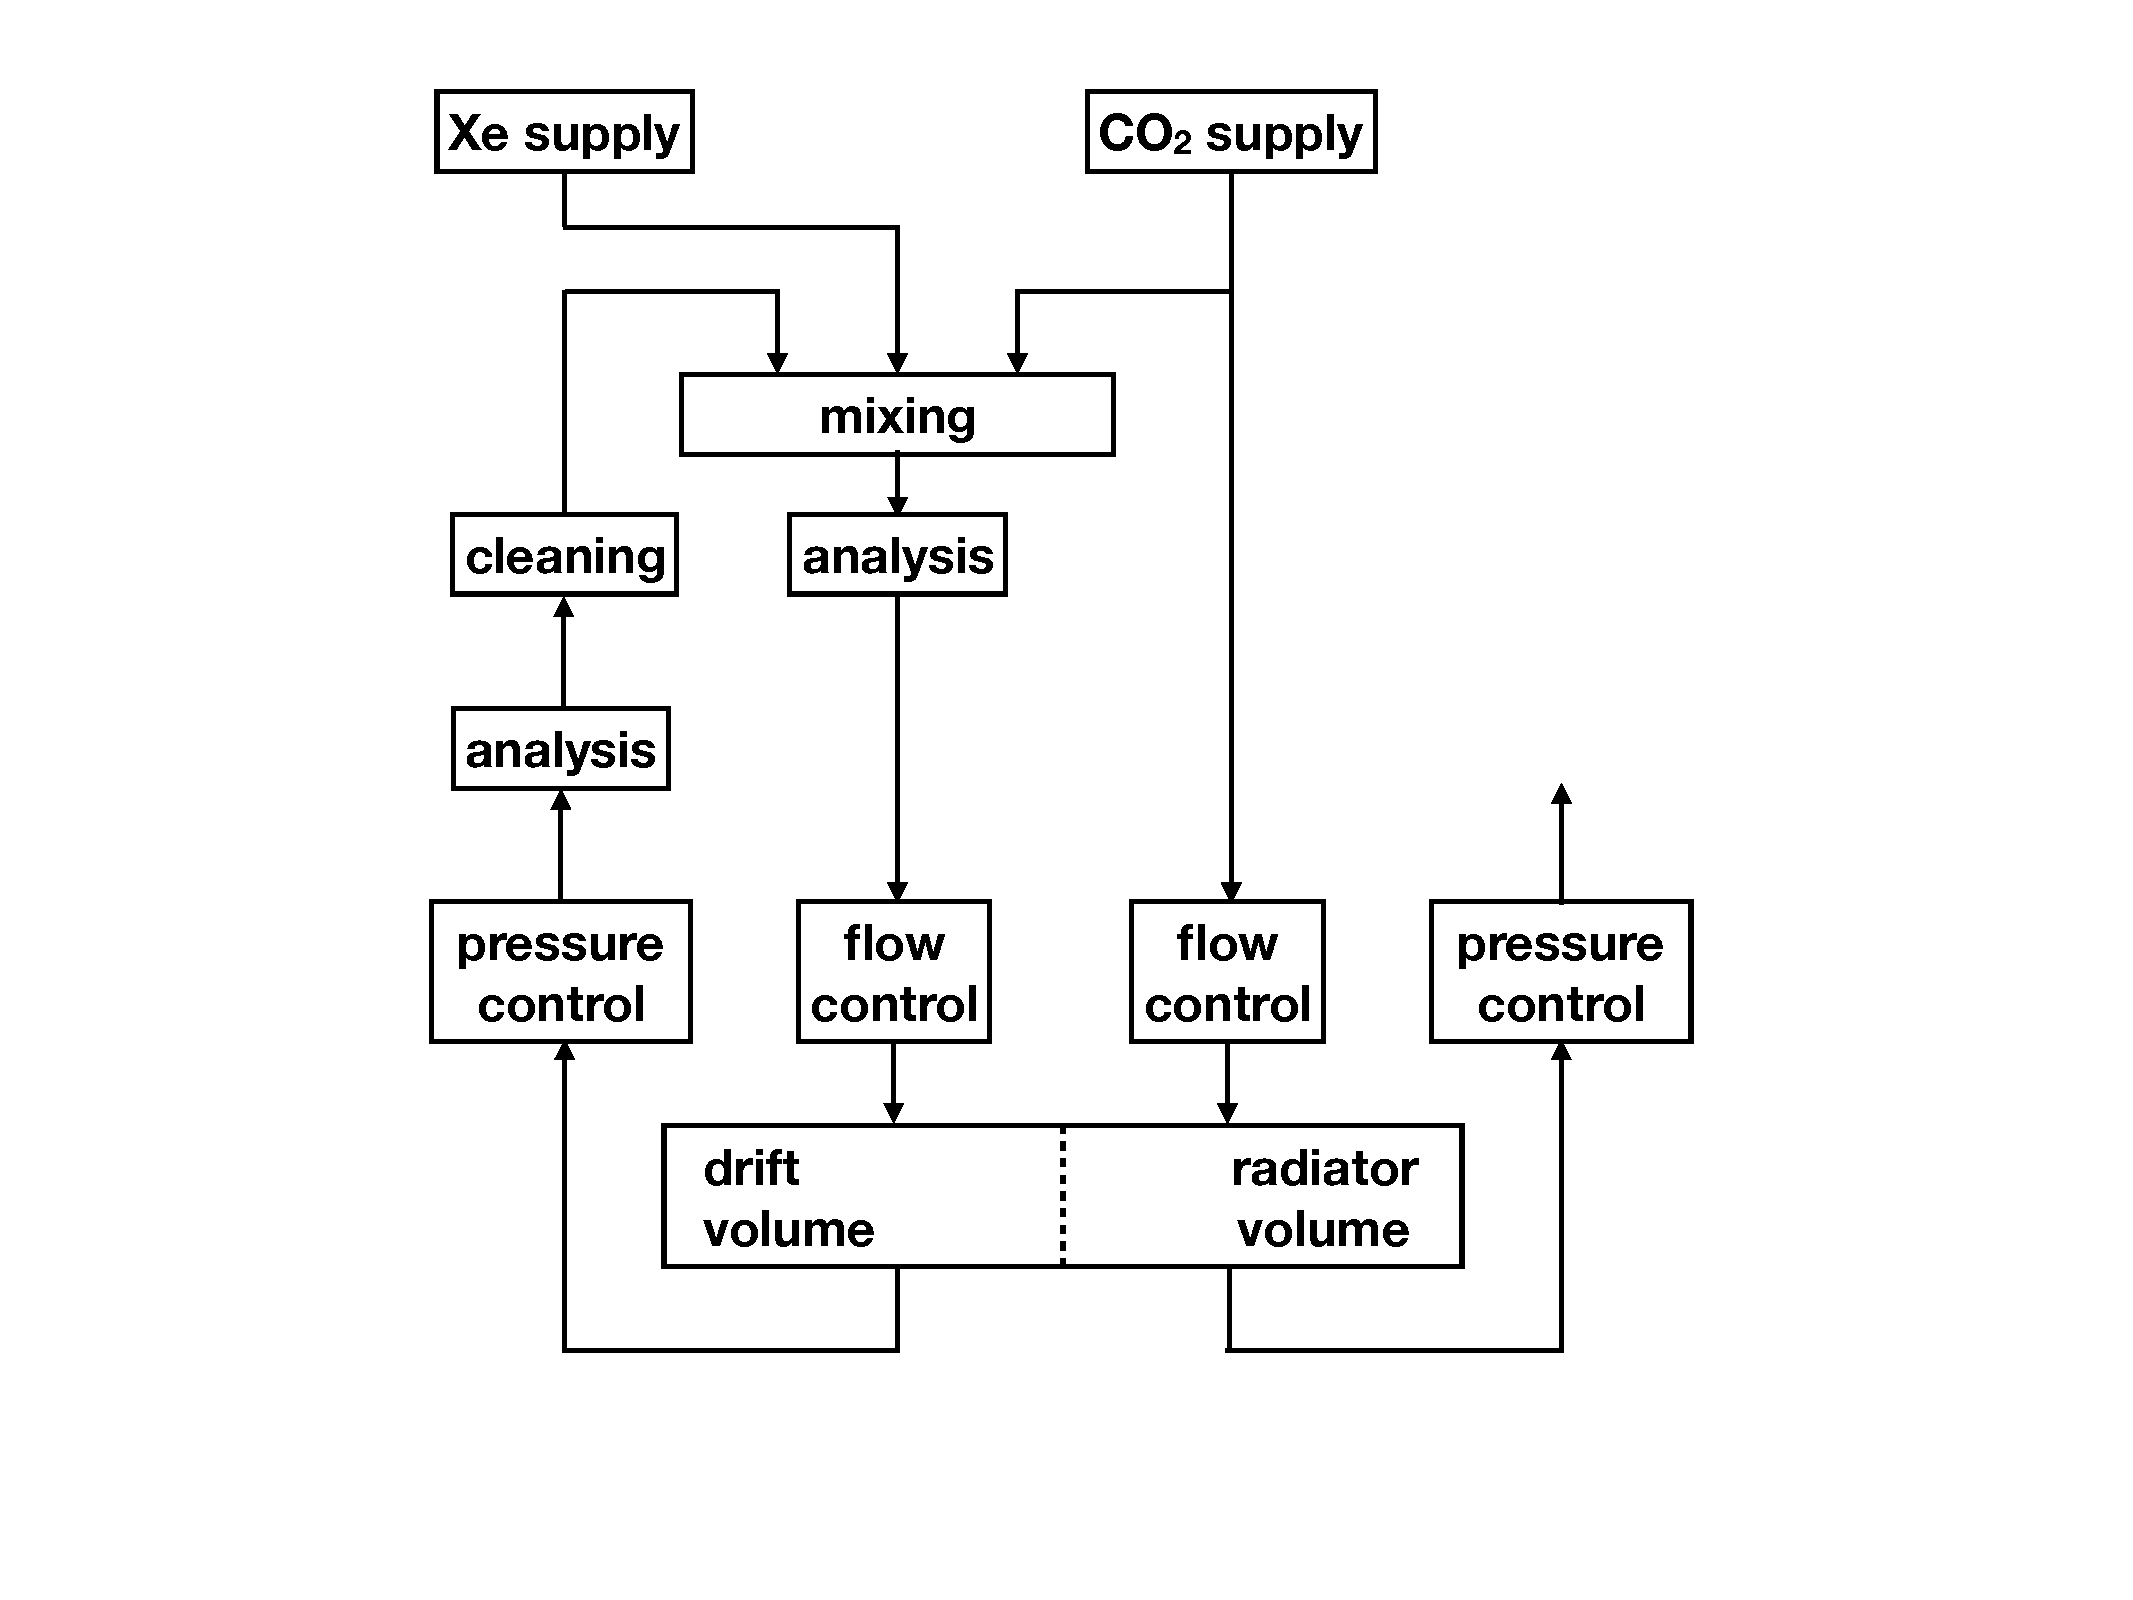
\includegraphics[width=0.80\textwidth]{./fig/TRD_gas_diagram-2175.pdf}
  \caption{
Principle diagram of the gas recirculating system.
}
  \label{fig:gas}
\end{figure}
Each GEM-TRD module has two gas volumes - 
the main one filled with $Xe/CO_2$ gas mixture of $90/10\%$ 
containing the drift and the amplification volumes,
and the second one for the radiator filled with CO2. 
The thickness of the drift and amplification volume is $20$~mm and $10$~mm respectively.
Thus, we estimate the $Xe/CO_2$ gas volume to be $25$~l per chamber, or $50$~l in total.
For the $CO_2$ volume it has a thickness of $150$~mm or $125$~l per module and $250$~l total.
For the $Xe/CO_2$ volume we aim to have 8 volume exchanges per day, i.e. $20$~l/h.
The $CO_2$ volume can be exchanged once  per day or $5$~l/h.

The entrance and exit gas windows will be made of $100$~$\mu$m Mylar, possibly enforced with Rochacell
material.
The detector will allow operation with overpressure between $0.5$ and $2$~mbar.
The two gas volumes will be separated by $50$~$\mu$m Mylar, covered with $1$~$\mu$m $Al$.
To limit the variations of the drift field, we require the pressure difference between the two gas
volumes to be less than $0.2$~mbar. 

Oxygen contamination and water vapor should be kept less than $50$~ppm, 
to minimize the electron recombination 
in the drift volume. The Nitrogen contamination should be kept less than $0.5\%$.

The elements of the gas system that operate above $1$~bar should be kept in a separate gas room,
elevated approximately $7$~m above the detector. They will be connected to the detector with
gas lines of about $50$~m length.

The parameters and requirements of the gas system are summarized in Table \ref{tab:gas}.

\begin{table}[h!]
\begin{ruledtabular}
\begin{tabular}{lcc}
\textrm{item}&
\textrm{requirement}&
\textrm{comment}\\
\colrule
total $Xe/CO_2$  gas volume & $50$ l &\\
total $CO_2$ gas volume & $250$ l &\\
$Xe/CO_2$  gas flow & $20$ l/h &\\
$CO_2$ gas flow & $5$ l/h &\\
Operating overpressure & $0.5-2$~mbar &\\
Pressure difference b/n two volumes & $<0.2$~mbar &\\
Oxygen contamination & $<50$~ppm &\\
water vapor & $<50$~ppm &\\
Nitrogen contamination & $<0.5\%$ &\\
\end{tabular}
\end{ruledtabular}
\caption{
General parameters and requirements for the GlueX TRD gas system.
\label{tab:gas}
}
\end{table}

\newpage
\section{Electronics}
We consider two options for the electronics.
We can use the same  electronics as for the GlueX drift chambers:
GASII \cite{GASII} preamps and flashADC-125 \cite{fADC125}.
......

The alternative is ...
.....

Comparison between the two
......

Cost estimates
......

(expect contribution from Sergey...)


\newpage
\section{Cost estimates and timeline}
\label{sec:time}
The estimated cost for the whole detector is summarized in Table.\ref{tab:cost}.
It is dominated by the electronics and the two options discussed
in the previous section are considered.
The price of the detector itself is based on the contract for producing the large scale 
prototype, and the experience of building large GEM chambers.
The gas system price was discussed with experts from CERN.
\begin{table}[h!]
\begin{ruledtabular}
\begin{tabular}{lcc}
\textrm{item}&
\textrm{price, \$k}&
\textrm{comment}\\
\colrule
electronics, option 1 (4,900 channels) & 490 & using existing pre-amp and fADC \\
electronics, option 2 (4,900 channels) & 245 & using modern design, under development \\
design and manufacture two TRD chambers  & 120 & \\
gas recirculating system  & 150 & \\
mechanical support and infrastructure  & 50 & \\
\colrule
total option 1 & 810 & \\
total option 2 & 565 & \\
\end{tabular}
\end{ruledtabular}
\caption{
Cost estimate for the whole GEM-TRD detector for two electronics options.
\label{tab:cost}
}
\end{table}

The general timeline of the proposed GEM-TRD project is shown in Table.\ref{tab:time}.
The prototyping with small detectors proved the principle of using GEM 
technology for TR detectors and helped to formulate the specifications for the next 
large-scale prototype.
A contract with UVA was signed to design and produce the large-scale prototype,
that we intend to test during the 2022-2023 running periods.
At the same time we plan to develop and produce the gas system.
Based on the result with the large prototype we will finalize the detector design.
The first chamber is planned to be manufactured and used during the phase-II
of the GlueX experiment in 2023-2025.
Even covering half of the acceptance, it will allow to measure  
the calorimeter rejection efficiency and evaluate the KF, which results
can be applied to the whole data set.
In 2025-2026 we plan to produce second chamber and finish the project.
\begin{table}[h!]
\begin{ruledtabular}
\begin{tabular}{lcc}
\textrm{year}&
\textrm{item}&
\textrm{comment}\\
\colrule
2018-2021 & tests with small prototypes & finished \\
2021-2023 & produce and test large-scale prototype & in progress \\
2022-2023 & design and produce gas system & \\
2023-2025 & produce and evaluate one chamber & use during GlueX phase-II \\
2025-2026 & produce and install the second chamber & 
\end{tabular}
\end{ruledtabular}
\caption{
General timeline of the GEM-TRD project.
\label{tab:time}
}
\end{table}


\section{Appendix}

Examples of the $p/E$ fits in bins of energy are given in 
Fig.\ref{fig:BCALbin47} for BCAL and in Fig.\ref{fig:FCALbin47} for FCAL.
\begin{figure}[h]
  \begin{subfigure}[b]{0.49\textwidth}
    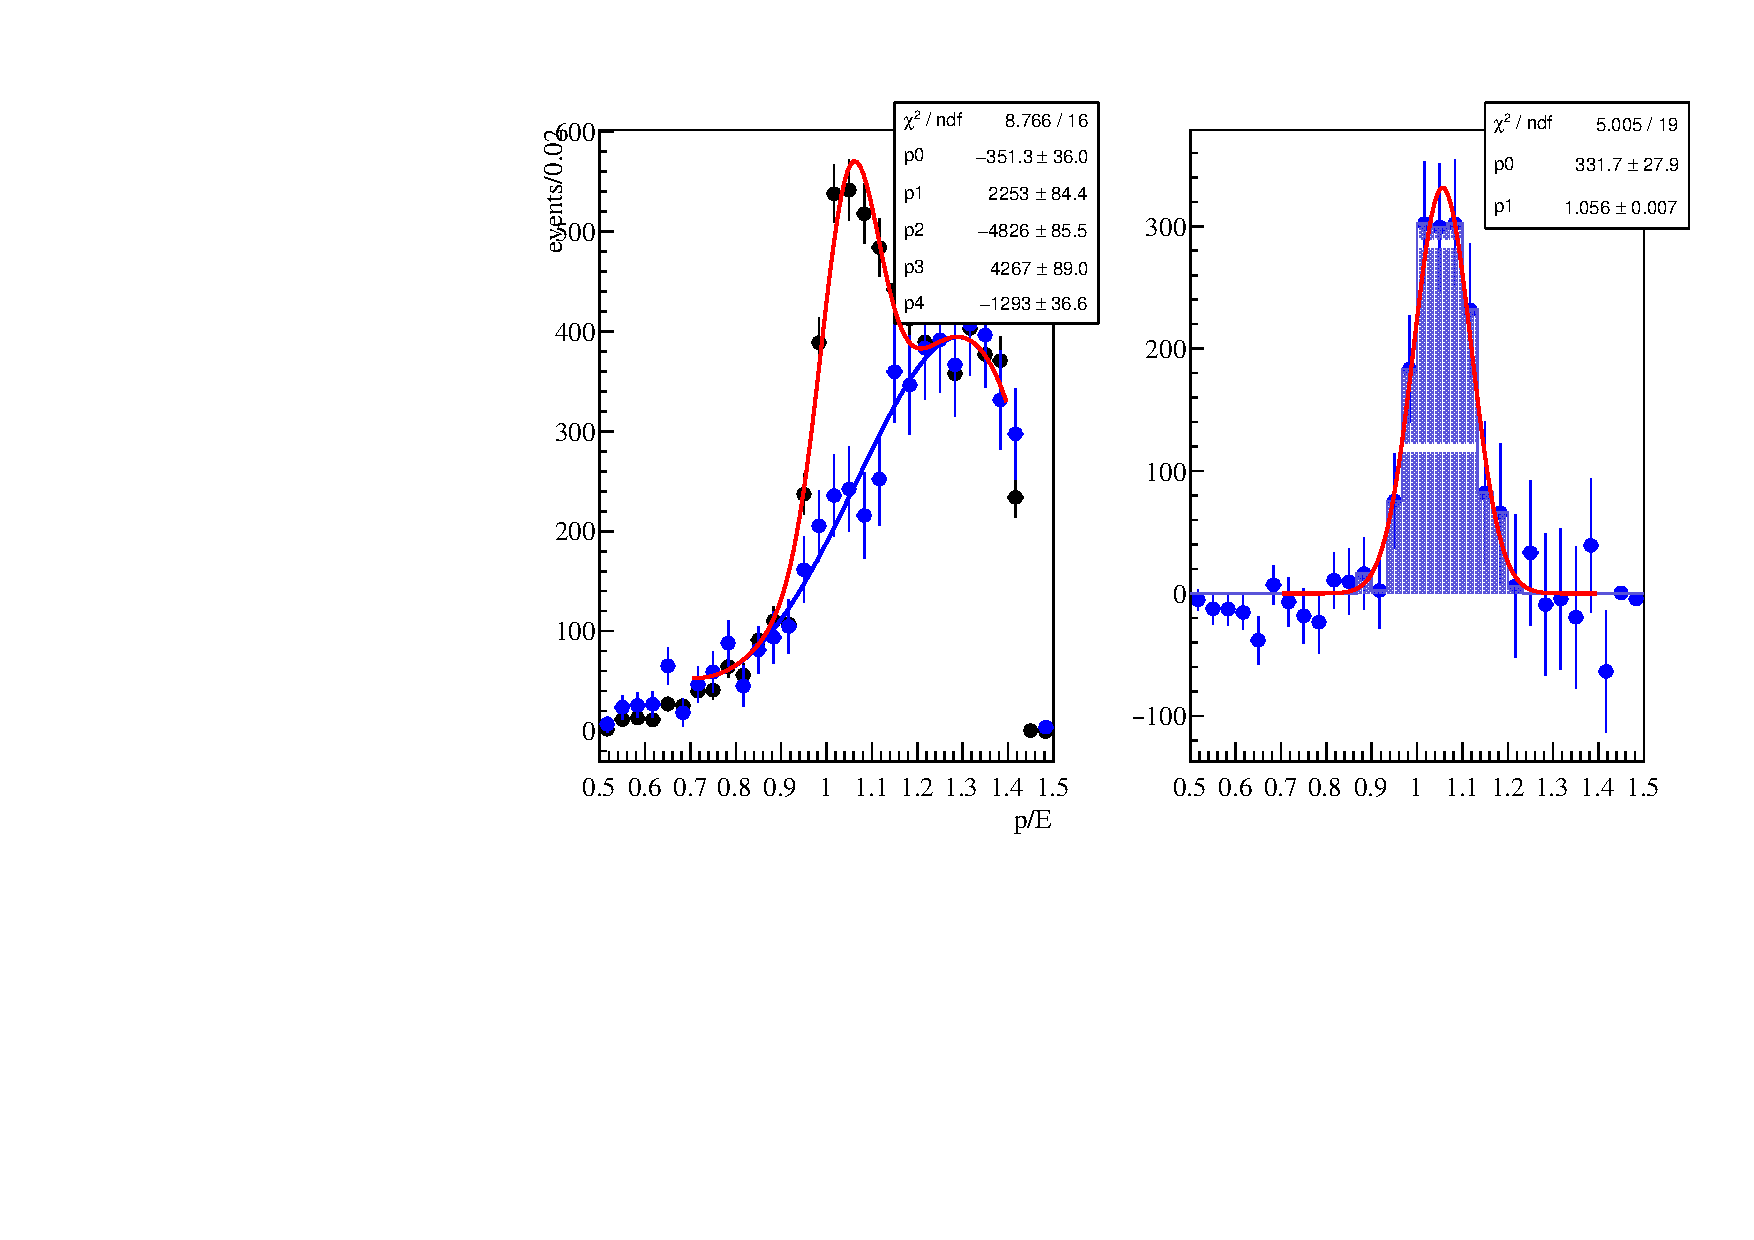
\includegraphics[width=\textwidth]{./fig/AN2_PovE_BCAL_bin4.pdf}
    \caption{BCAL bin 4 $8.74<E_\gamma <8.92$ GeV }
    \label{fig:BCALbin4}
  \end{subfigure}
  %
  \begin{subfigure}[b]{0.49\textwidth}
    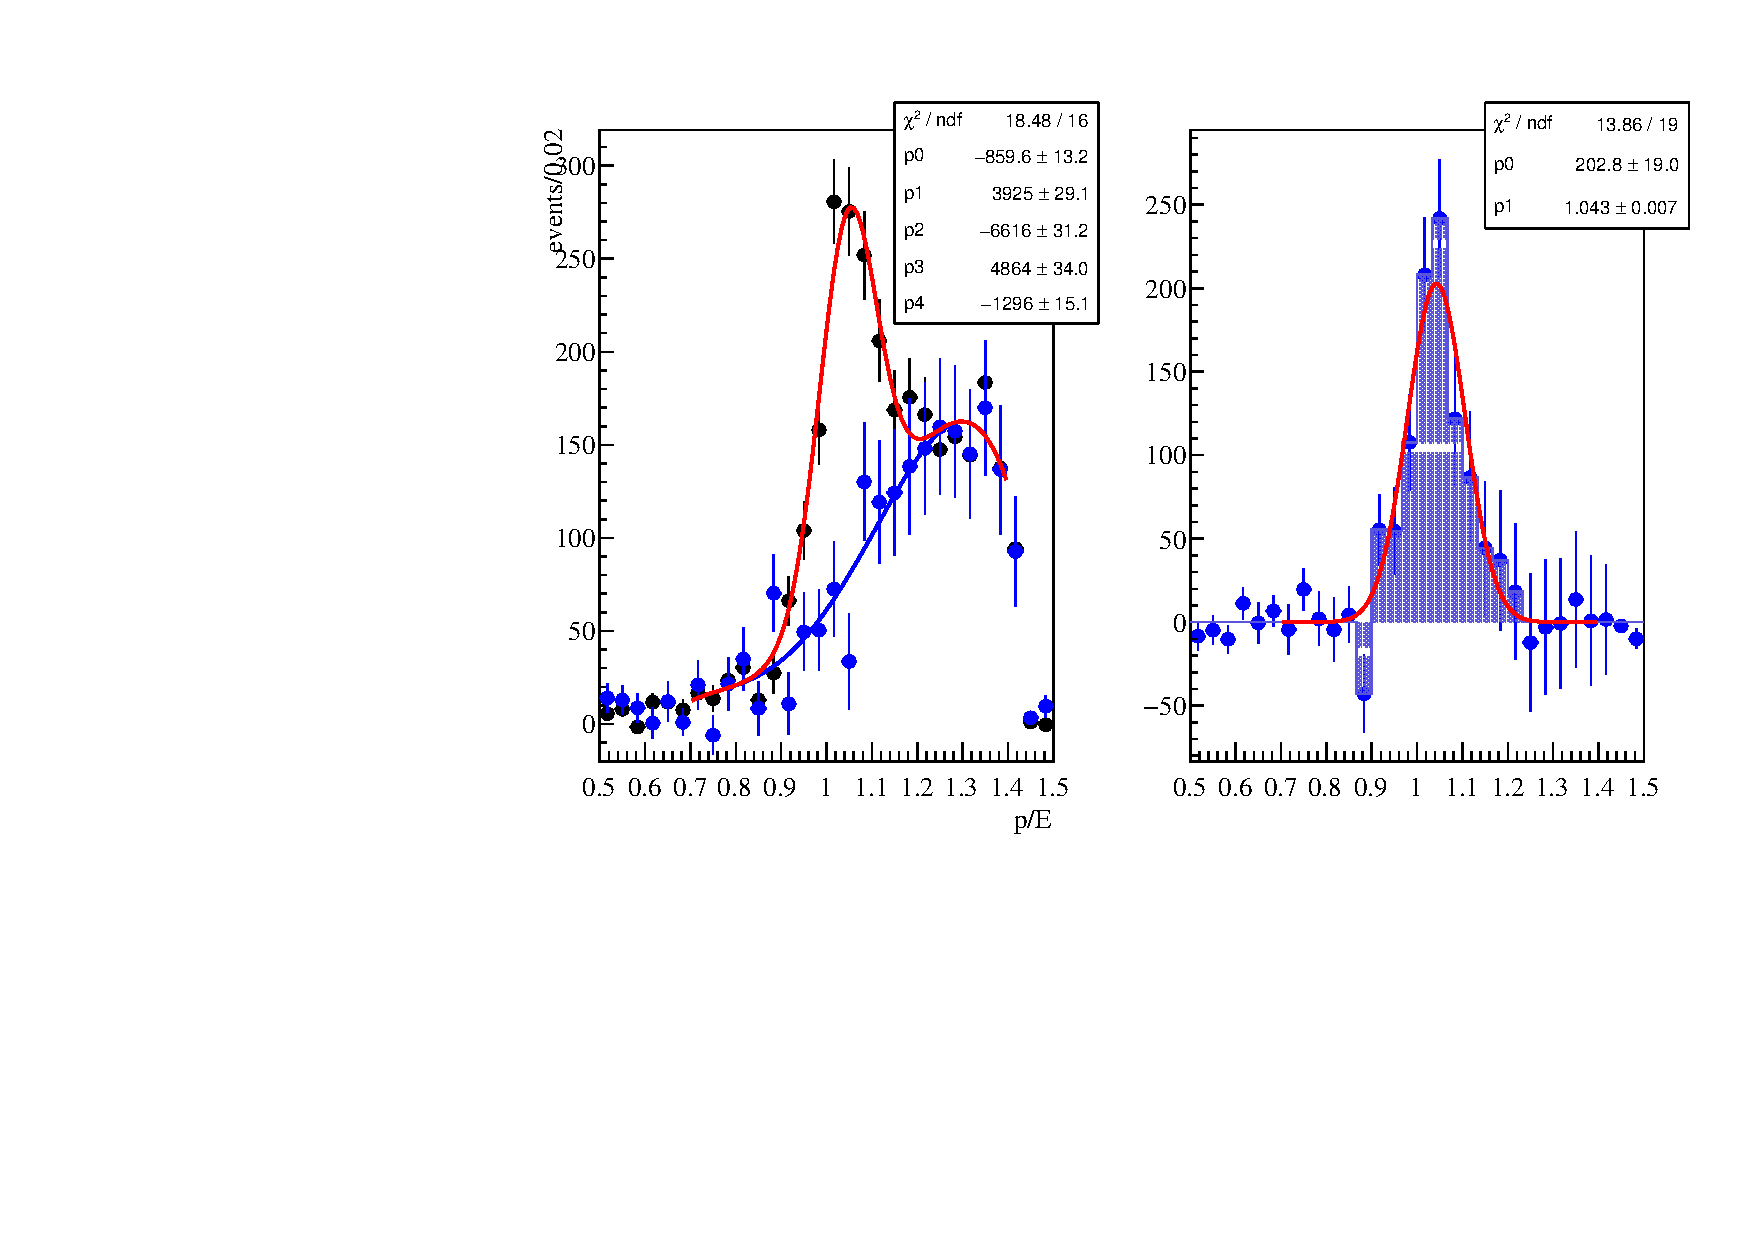
\includegraphics[width=\textwidth]{./fig/AN2_PovE_BCAL_bin5.pdf}
    \caption{BCAL bin 5 $8.92<E_\gamma <9.10$ GeV }
    \label{fig:BCALbin5}
  \end{subfigure}
  \begin{subfigure}[b]{0.49\textwidth}
    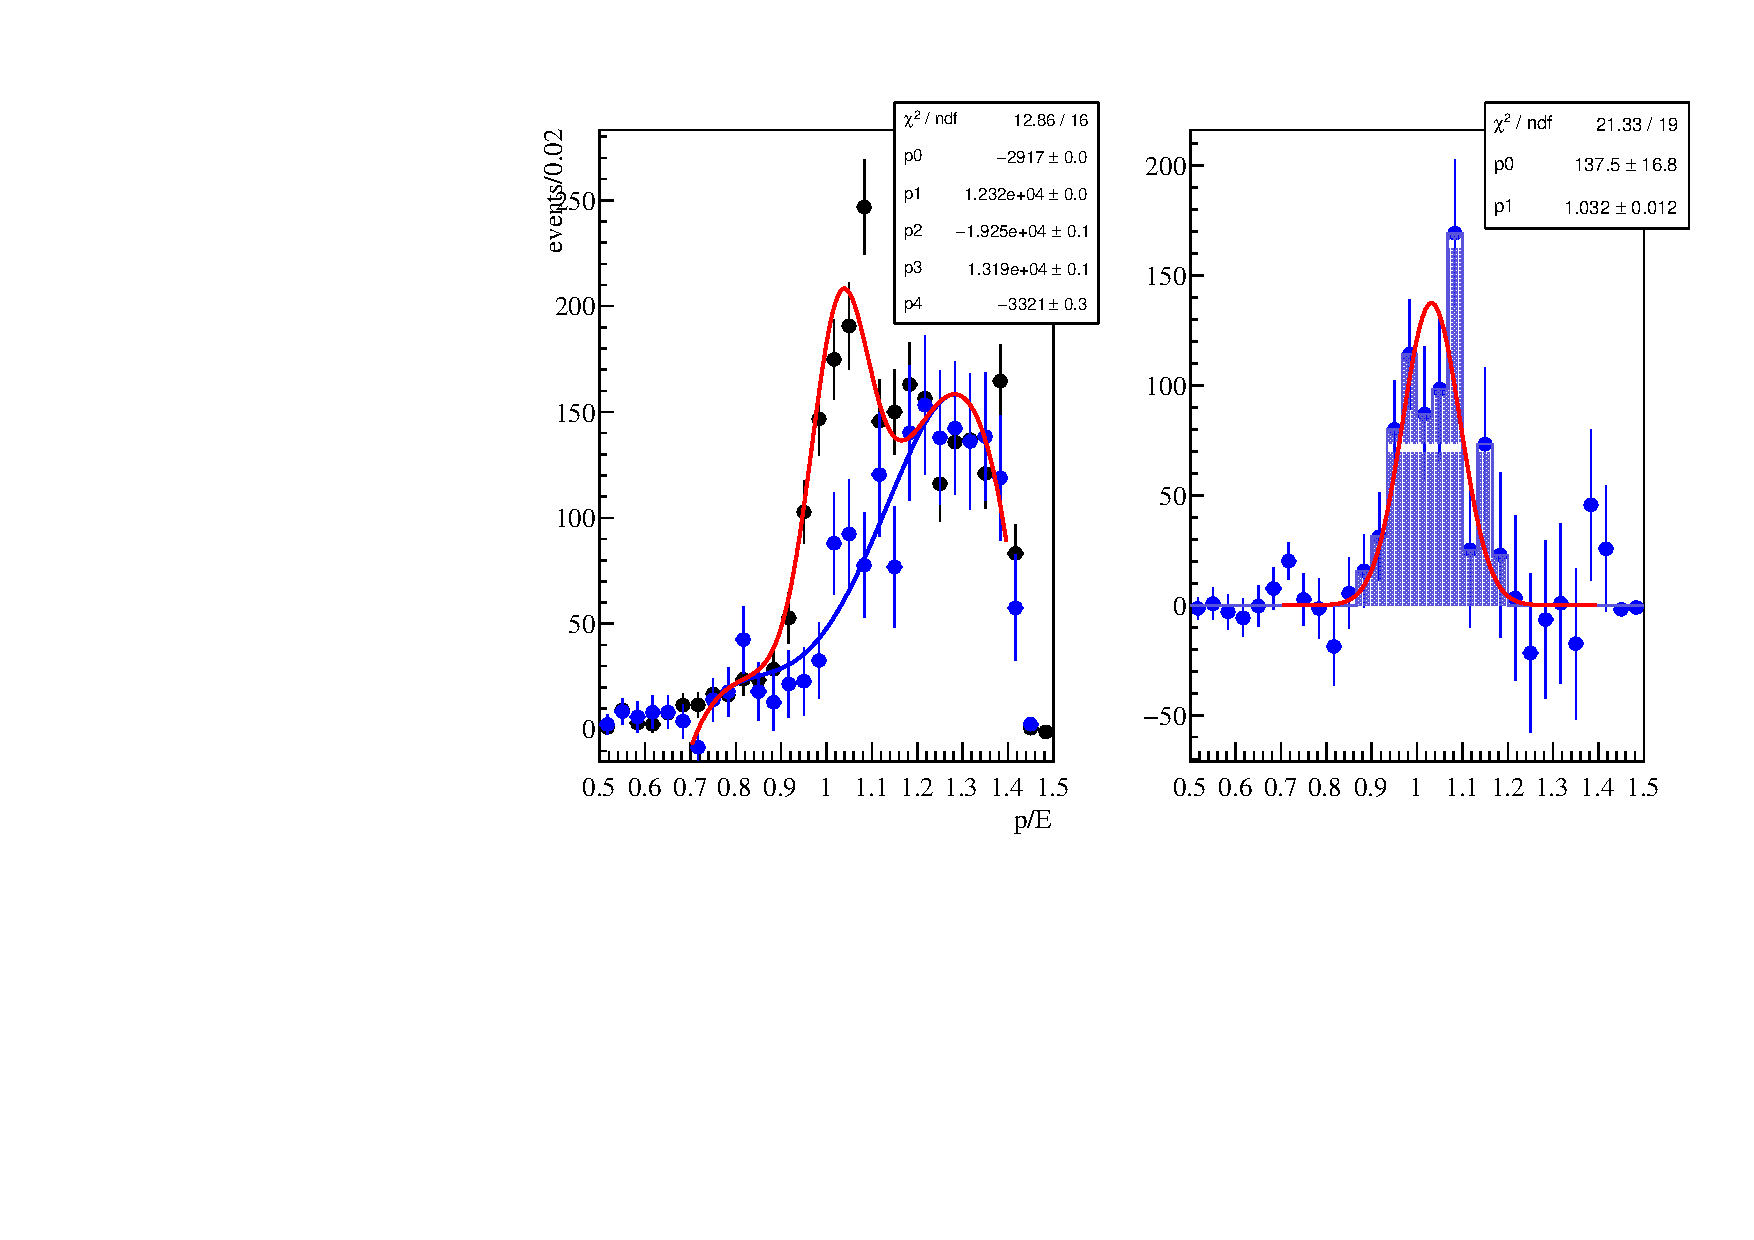
\includegraphics[width=\textwidth]{./fig/AN2_PovE_BCAL_bin6.pdf}
    \caption{BCAL bin 6 $9.10<E_\gamma <9.28$ GeV }
    \label{fig:BCALbin6}
  \end{subfigure}
  %
  \begin{subfigure}[b]{0.49\textwidth}
    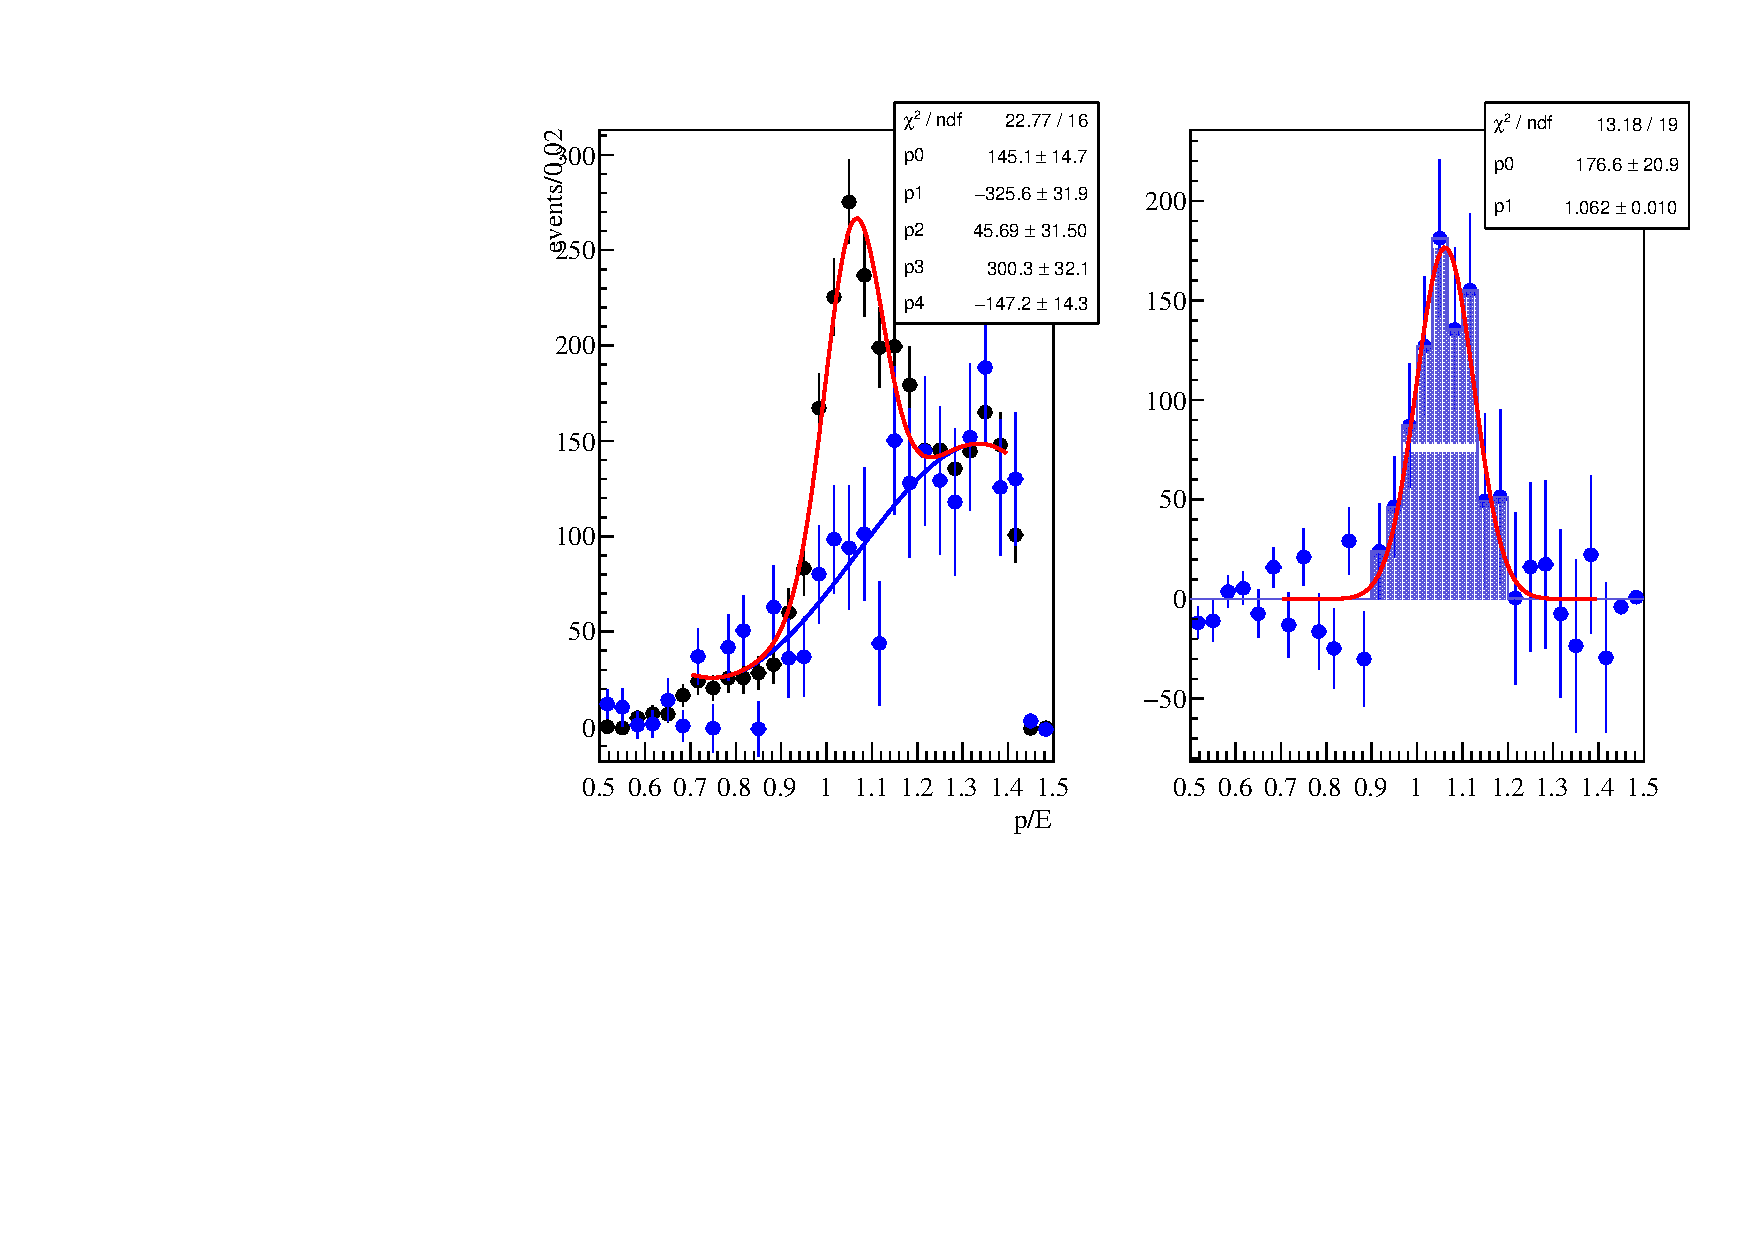
\includegraphics[width=\textwidth]{./fig/AN2_PovE_BCAL_bin7.pdf}
    \caption{BCAL bin 7 $9.28<E_\gamma <9.46$ GeV}
    \label{fig:BCALbin7}
  \end{subfigure}
  \caption{
Fits of $p/E$ distributions for BCAL for four energy bins.
% around the dip.
In the left panel of each plot the blue points fitted with the blue curve represent the
background distribution, while the total distribution is shown with black points
fitted with a Gaussian (fixed $\sigma $) plus the background polynomial (p0-p4 parameters);
the three fitted parameters are the normalization coefficients of the Gaussian and the polynomial and the mean of the Gaussian.
The right panel is the difference between the black and blue points from the left panel,
fitted with a Gaussian with fixed width (p0, p1 - amplitude and mean); the sum of the shaded points ($\pm 3\sigma $)
is used as an estimate of the signal.
}\label{fig:BCALbin47}
\end{figure}

\begin{figure}[h]
  \begin{subfigure}[b]{0.49\textwidth}
    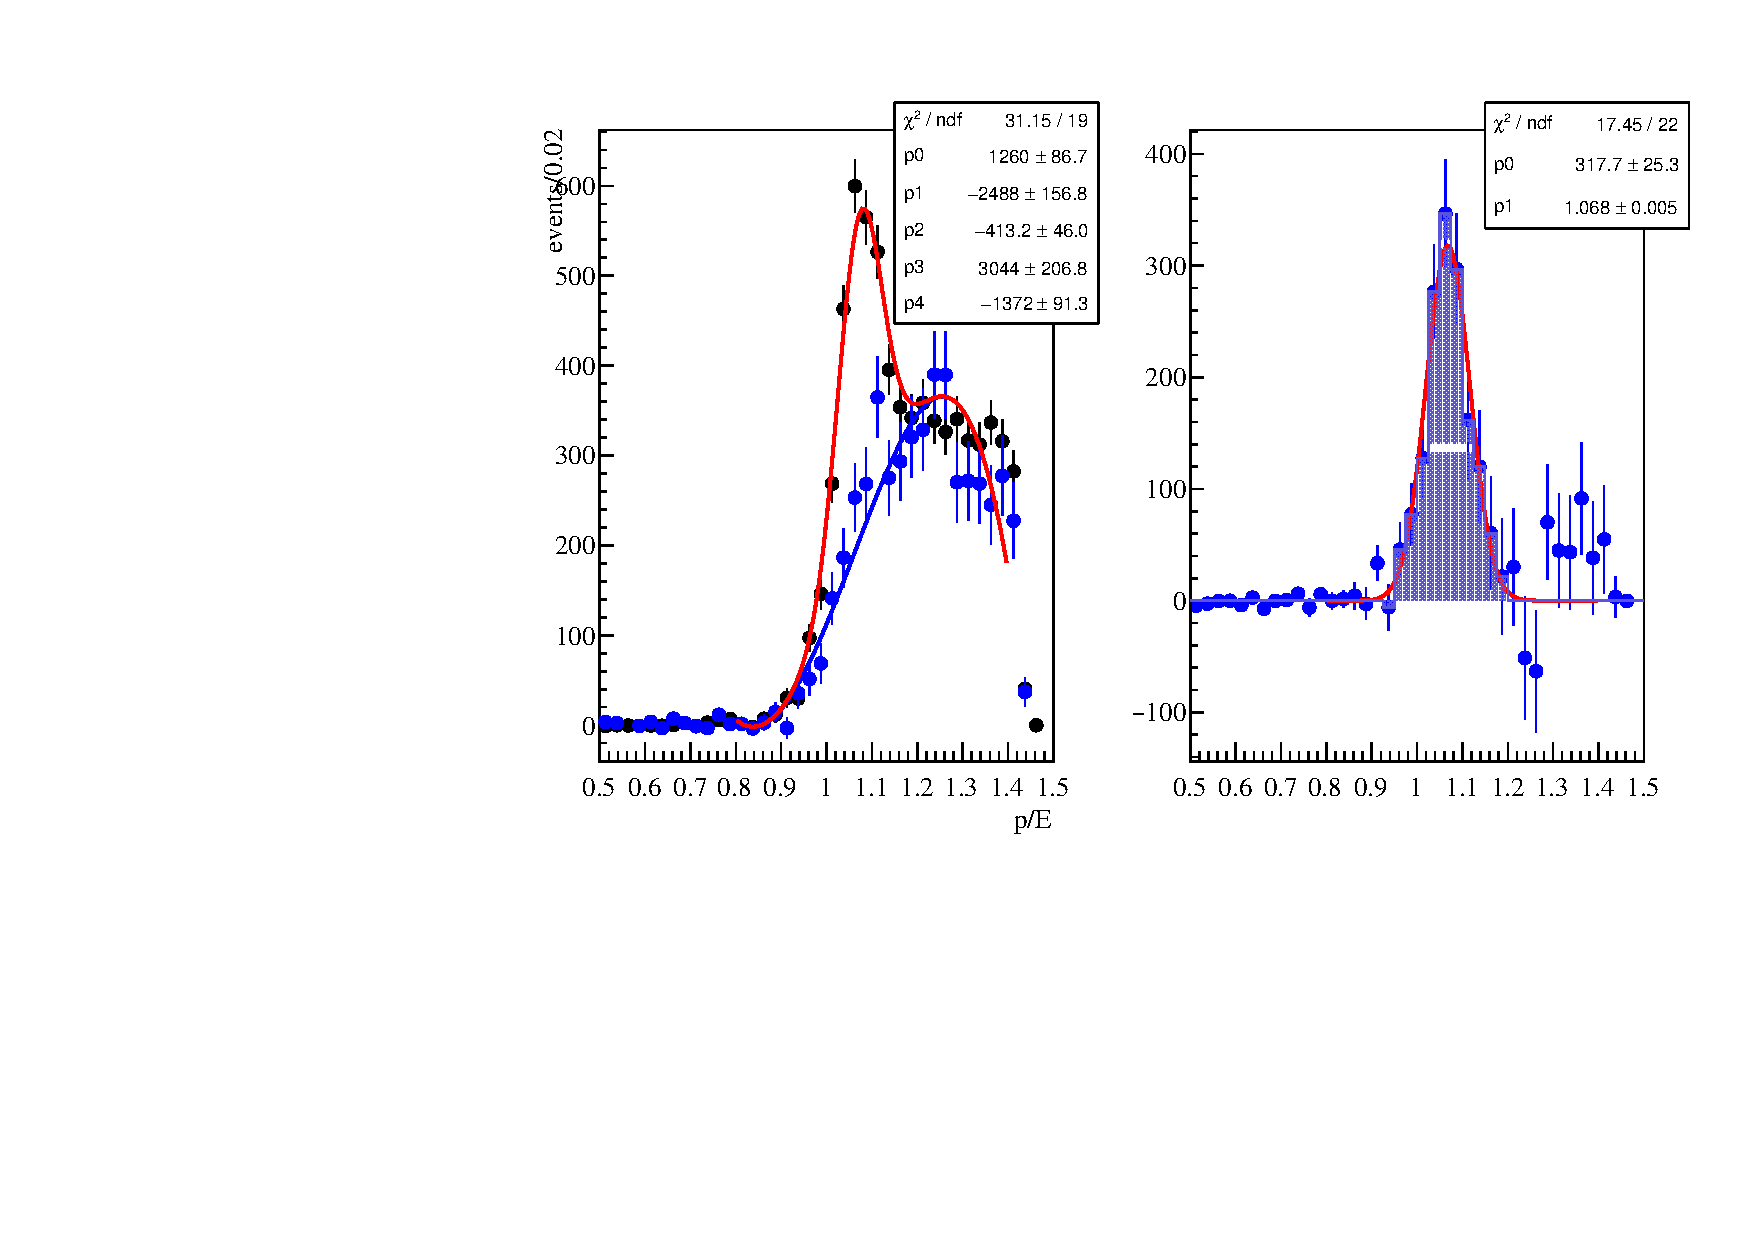
\includegraphics[width=\textwidth]{./fig/AN2_PovE_FCAL_bin4.pdf}
    \caption{FCAL bin 4 $8.74<E_\gamma <8.92$ GeV}
    \label{fig:FCALbin4}
  \end{subfigure}
  %
  \begin{subfigure}[b]{0.49\textwidth}
    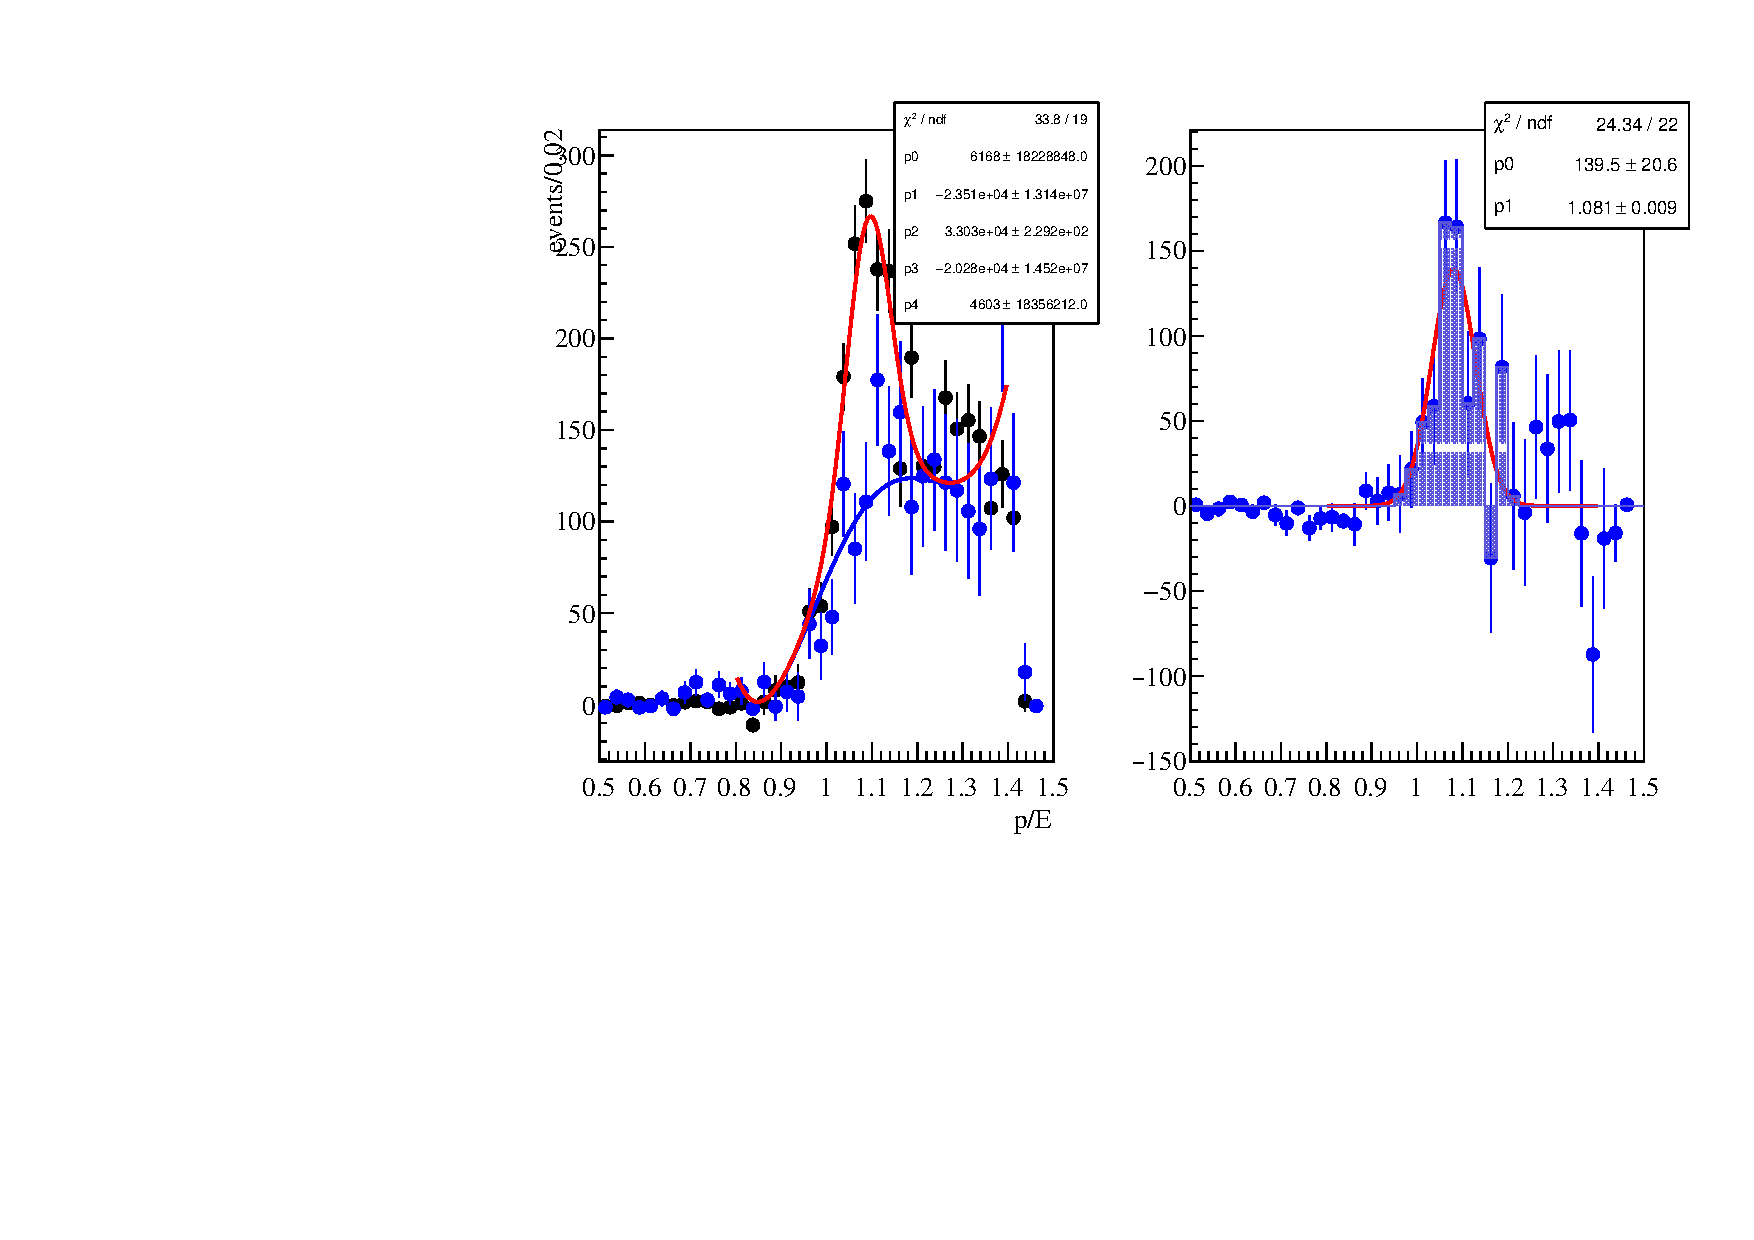
\includegraphics[width=\textwidth]{./fig/AN2_PovE_FCAL_bin5.pdf}
    \caption{FCAL bin 5 $8.92<E_\gamma <9.10$ GeV}
    \label{fig:FCALbin5}
  \end{subfigure}
  \begin{subfigure}[b]{0.49\textwidth}
    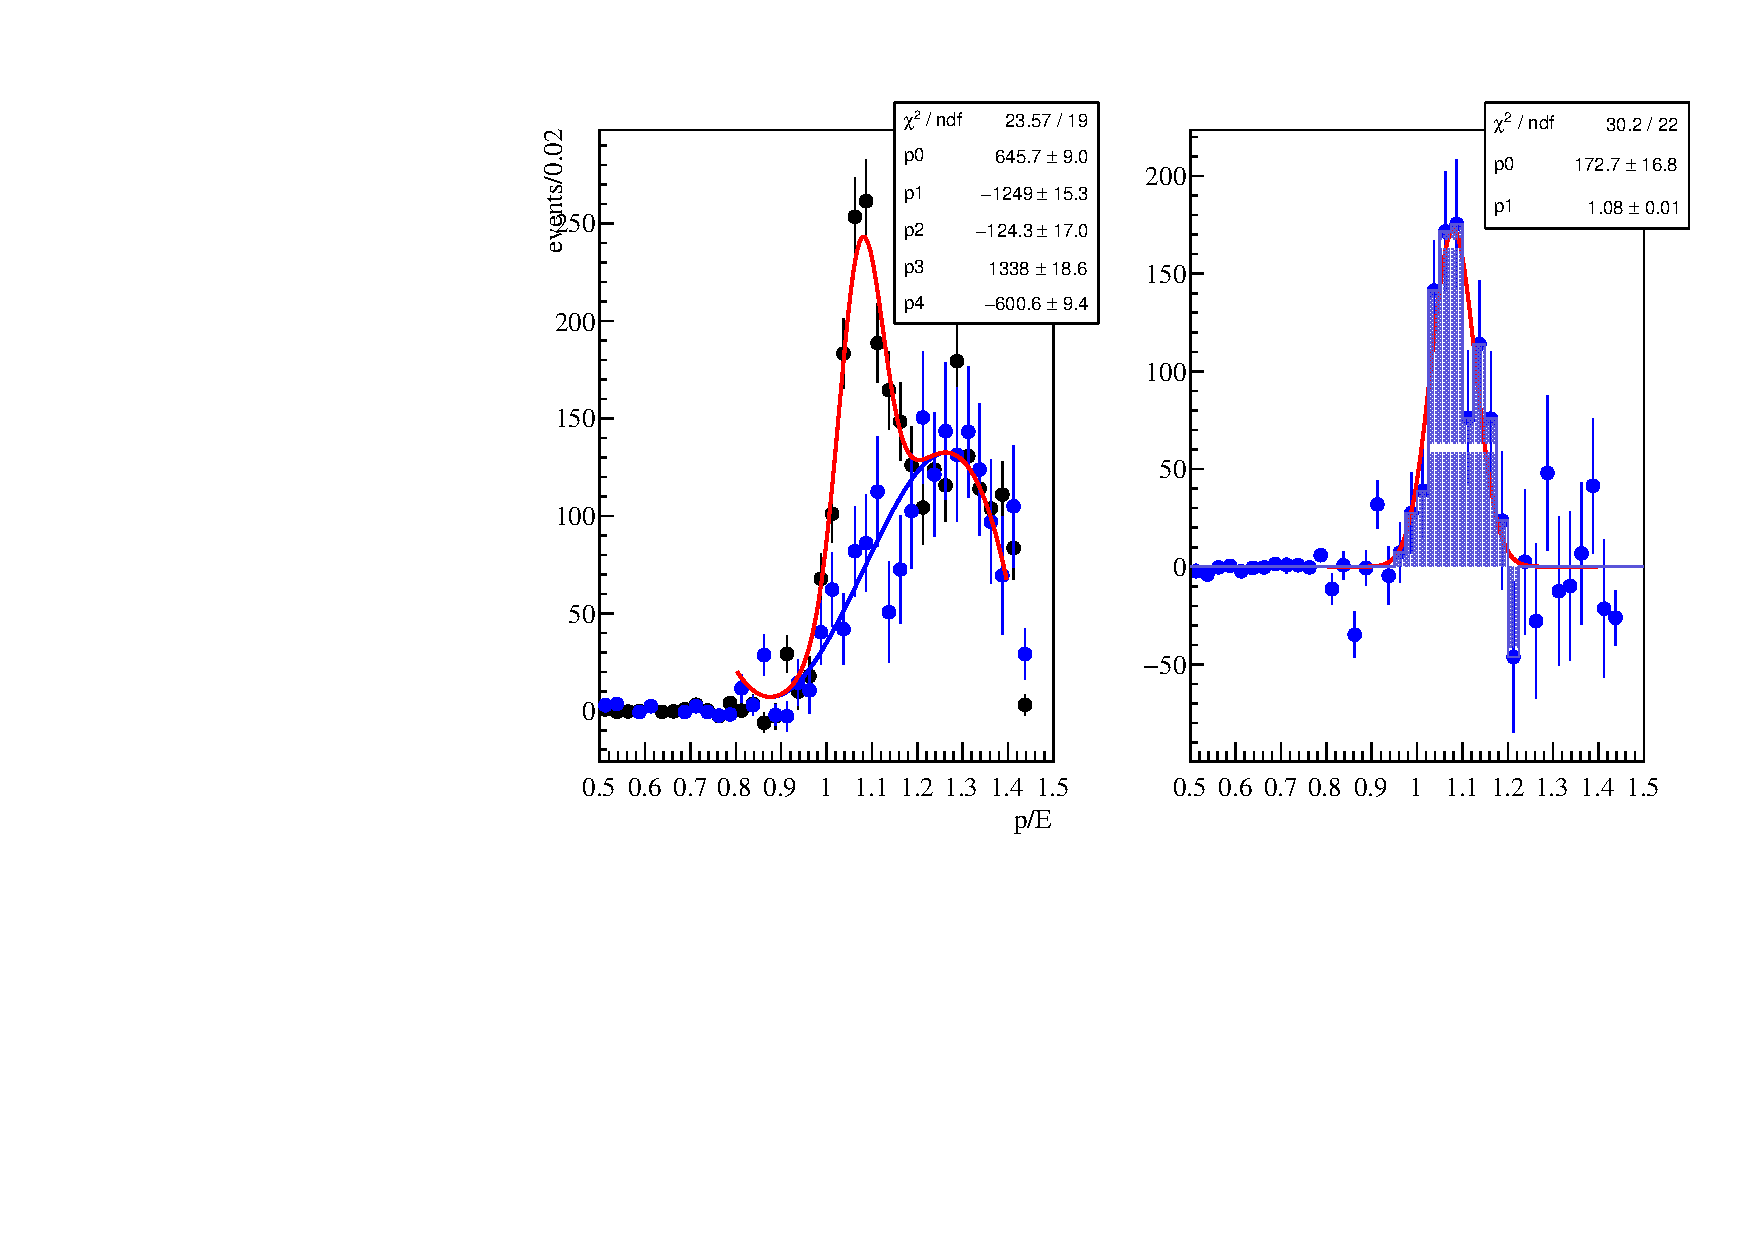
\includegraphics[width=\textwidth]{./fig/AN2_PovE_FCAL_bin6.pdf}
    \caption{FCAL bin 6 $9.10<E_\gamma <9.28$ GeV}
    \label{fig:FCALbin6}
  \end{subfigure}
  %
  \begin{subfigure}[b]{0.49\textwidth}
    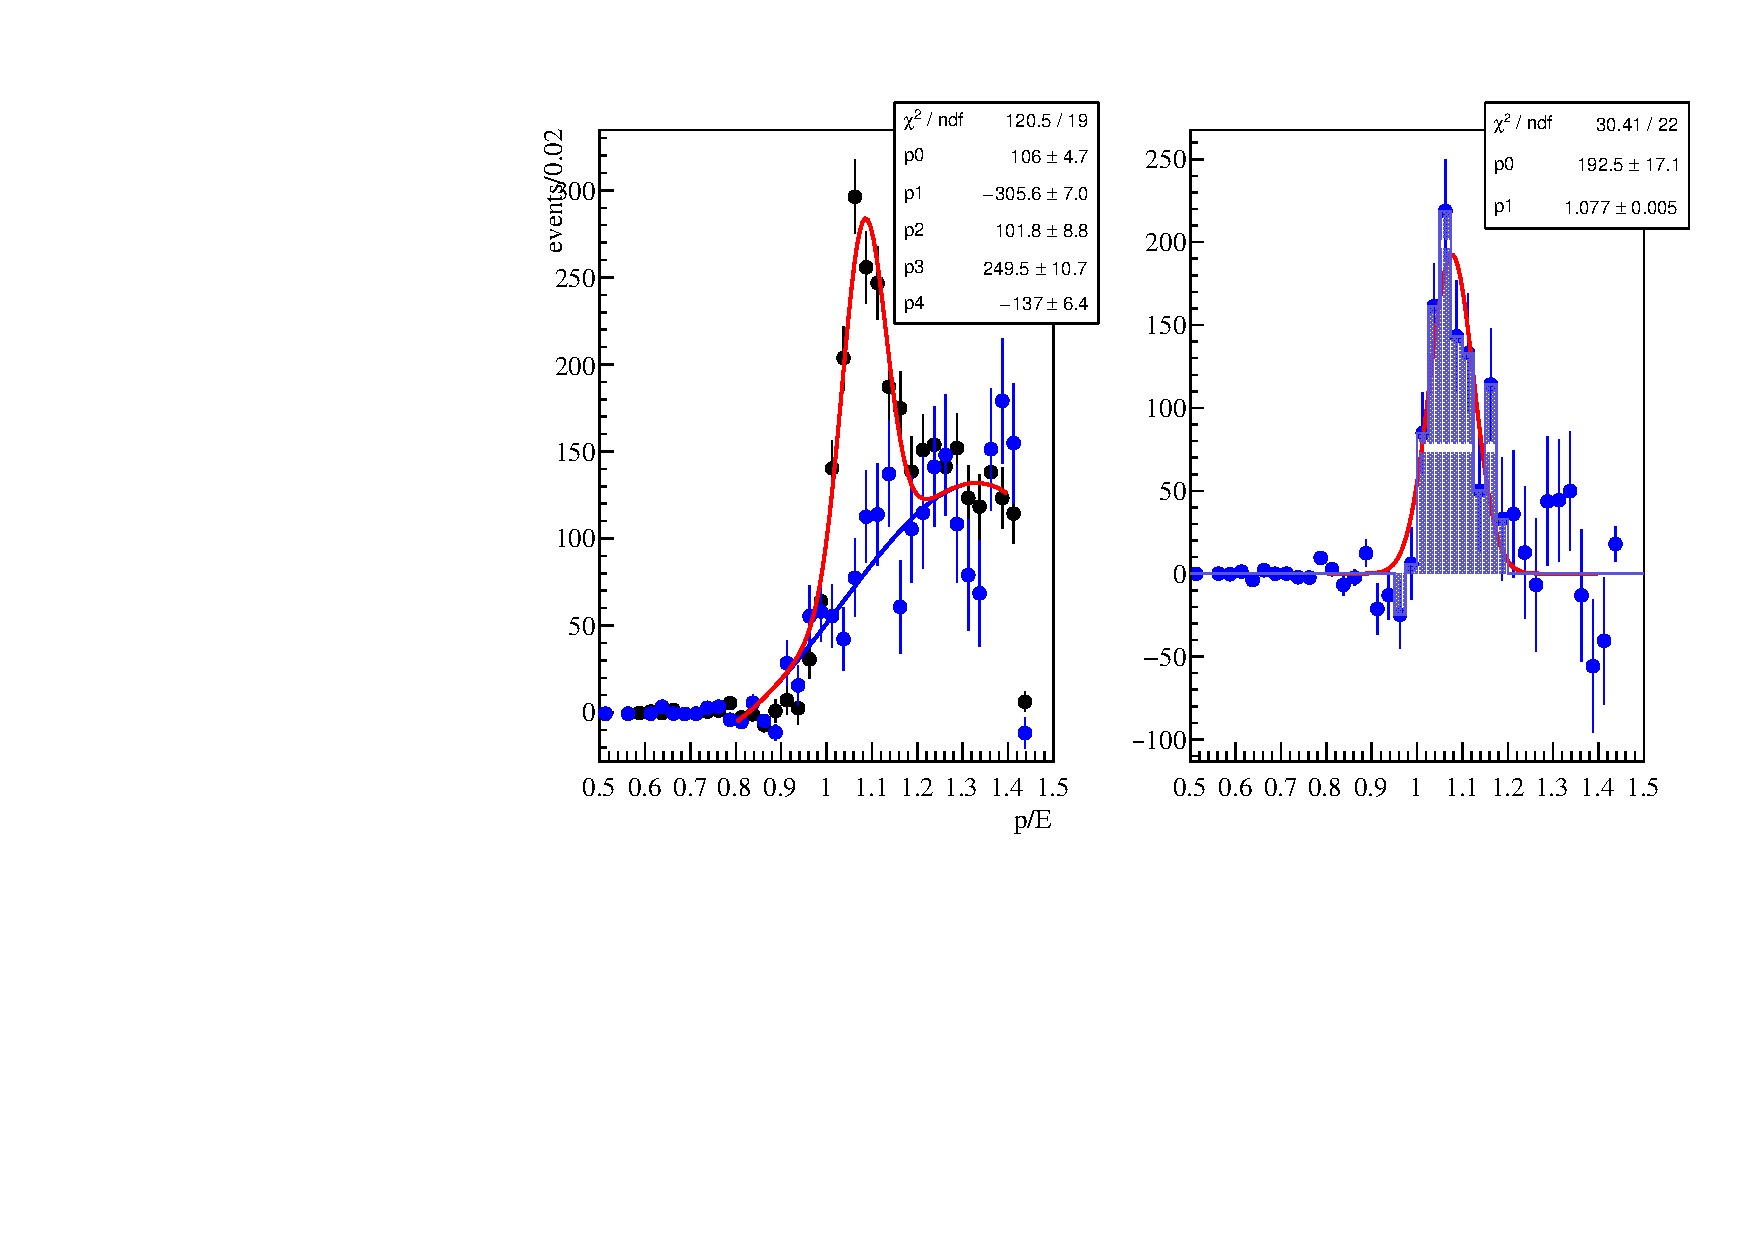
\includegraphics[width=\textwidth]{./fig/AN2_PovE_FCAL_bin7.pdf}
    \caption{FCAL bin 7 $9.28<E_\gamma <9.46$ GeV}
    \label{fig:FCALbin7}
  \end{subfigure}
  \caption{
Same as in Fig.\ref{fig:BCALbin47} but for FCAL.
}\label{fig:FCALbin47}
\end{figure}


\bibliography{gem_trd.bib}% Produces the bibliography via BibTeX.

\end{document}
%
% ****** End of file apssamp.tex ******
